\documentclass[10pt]{beamer}
\usetheme{Malmoe}
\colorlet{beamer@blendedblue}{green!40!black}
\setbeamertemplate{navigation symbols}{}
\newcommand*\oldmacro{}%
\let\oldmacro\insertshorttitle%
\renewcommand*\insertshorttitle{%
\oldmacro\hfill%
\insertframenumber\,/\,\inserttotalframenumber}

\usepackage{caption}
\usepackage{hyperref}
\usepackage[makeroom]{cancel}
\usepackage{ amssymb }
\usepackage{appendixnumberbeamer}
%\usepackage{tikz-feynman}

\usepackage{xfrac}
\usepackage{graphicx}
\begin{document}
\title[Search for $t\rightarrow q\gamma$ in Top Pair Events \hfill]{Search for the Flavor Changing Neutral Current, $t\rightarrow q \gamma$ in Top Pair Events Using the ATLAS Detector}
\author[Barkeloo, Defense]{Jason Barkeloo}

\titlegraphic{\hspace*{6.75cm}~%
   
\includegraphics[width=4cm]{../uo_logo_green_on_white_2.jpg}
}

%\frame{\frametitle{}
%\begin{itemize}
%\item
%\end{itemize}
%}


\date{April 16, 2020}
\frame{\titlepage}
\frame{\frametitle{Welcome!}
Thank you for your flexibility given our current situation! \\~\

Defense proceedings:
\begin{itemize}
\item Open/public presentation in this room with followup questions
\item Committee and myself will adjourn to a separate room to conclude
\item Committee will deliberate and I will return to this room \\~\
\end{itemize}

General Guidelines:
\begin{itemize}
\item Please mute if not speaking  \\~\
\end{itemize}

\centering
\textbf{Thank you for attending!}
}

\frame{\frametitle{Overview}\tableofcontents[hideallsubsections]}%hidesubsections]}
\section{Background}
%\frame{\frametitle{Table of Contents}\tableofcontents[currentsection,hideothersubsections]}
%%%%%%%%%%%%%%%%%%%%%%%%%%%%%%%%%%%%%%%%%%%%%%%%%%%%%%%%%
\subsection{The Standard Model}
\frame{\frametitle{The Standard Model}
\begin{figure}
	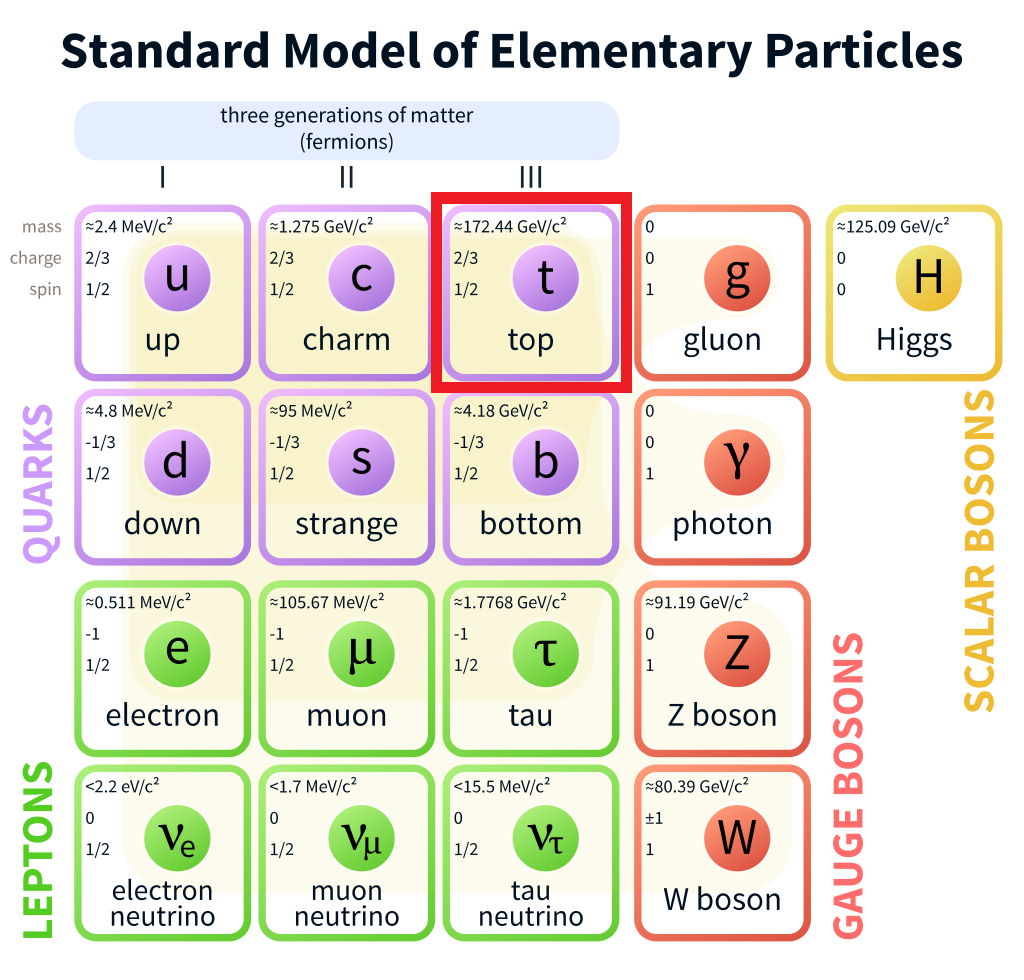
\includegraphics[width=4.8cm]{Images/SMParticles.png}
	%\captionof{figure}{\href{https://en.wikipedia.org/wiki/Standard_Model}{List of standard model particles}}
\end{figure}
\begin{itemize}
\item Best working description of fundamental particles and their interactions
	\begin{itemize}
	\item Experimentally precise and well behaved
	\end{itemize}
	
	\vspace{\baselineskip}
\end{itemize}
}

\subsection{The Top Quark}

\frame{\frametitle{The Top Quark}
\begin{itemize}
\item Heaviest fundamental particle, $172.5 GeV$
\item Lifetime $5x10^{-25}s$, decays before hadronization
	\begin{itemize}
	\item Allows us to study the decay of a single quark
	\end{itemize}
\end{itemize}
\begin{figure}
	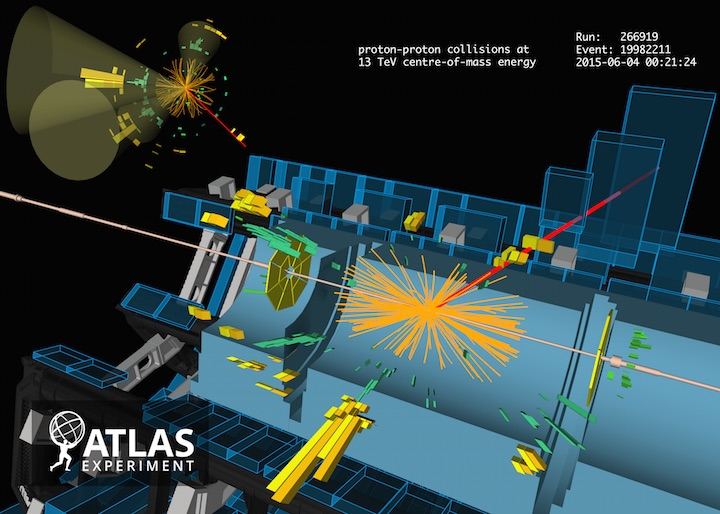
\includegraphics[height=0.5\textheight]{../../Thesis/ThesisImages/ttbarevent.jpg}
\end{figure}
}

\frame{\frametitle{Top Quark Pair Production}
\begin{itemize}
\item Leading order processes for top quark production
	\begin{itemize}
	\item Quark-antiquark annihilation $\approx 10\%$
	\item Gluon-gluon fusion $\approx 90\%$
	\end{itemize}
\end{itemize}
\centering

	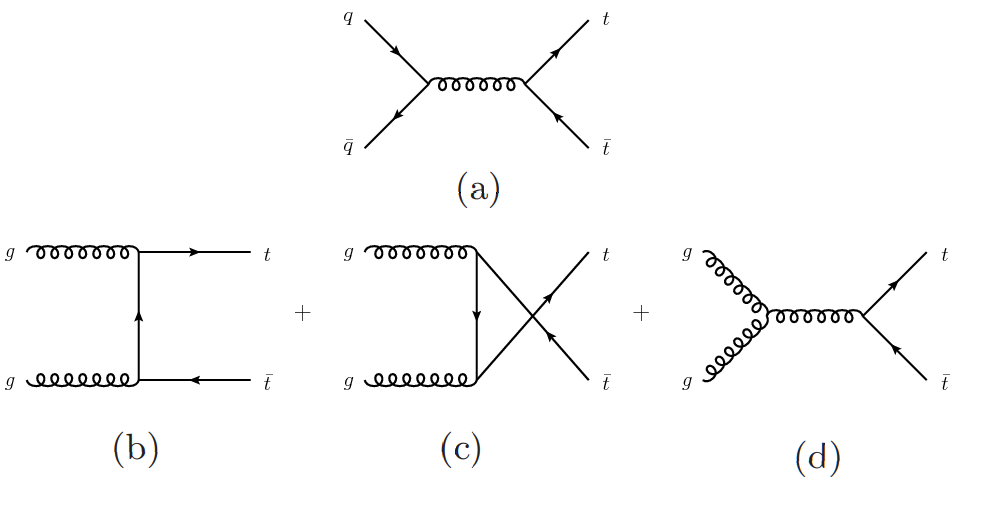
\includegraphics[height=0.5\textheight]{../../Thesis/ThesisImages/Theory/LOPairProdDiags.png}
	\captionof{figure}{Leading order $t\bar{t}$ diagrams}
}
\frame{\frametitle{Top Quark Pair Production}
\begin{itemize}
\item At $\sqrt{s}=13TeV$ for $m_{t}=172.5GeV$, $\sigma_{t\bar{t}} = 831.76pb$
\end{itemize}
\centering
	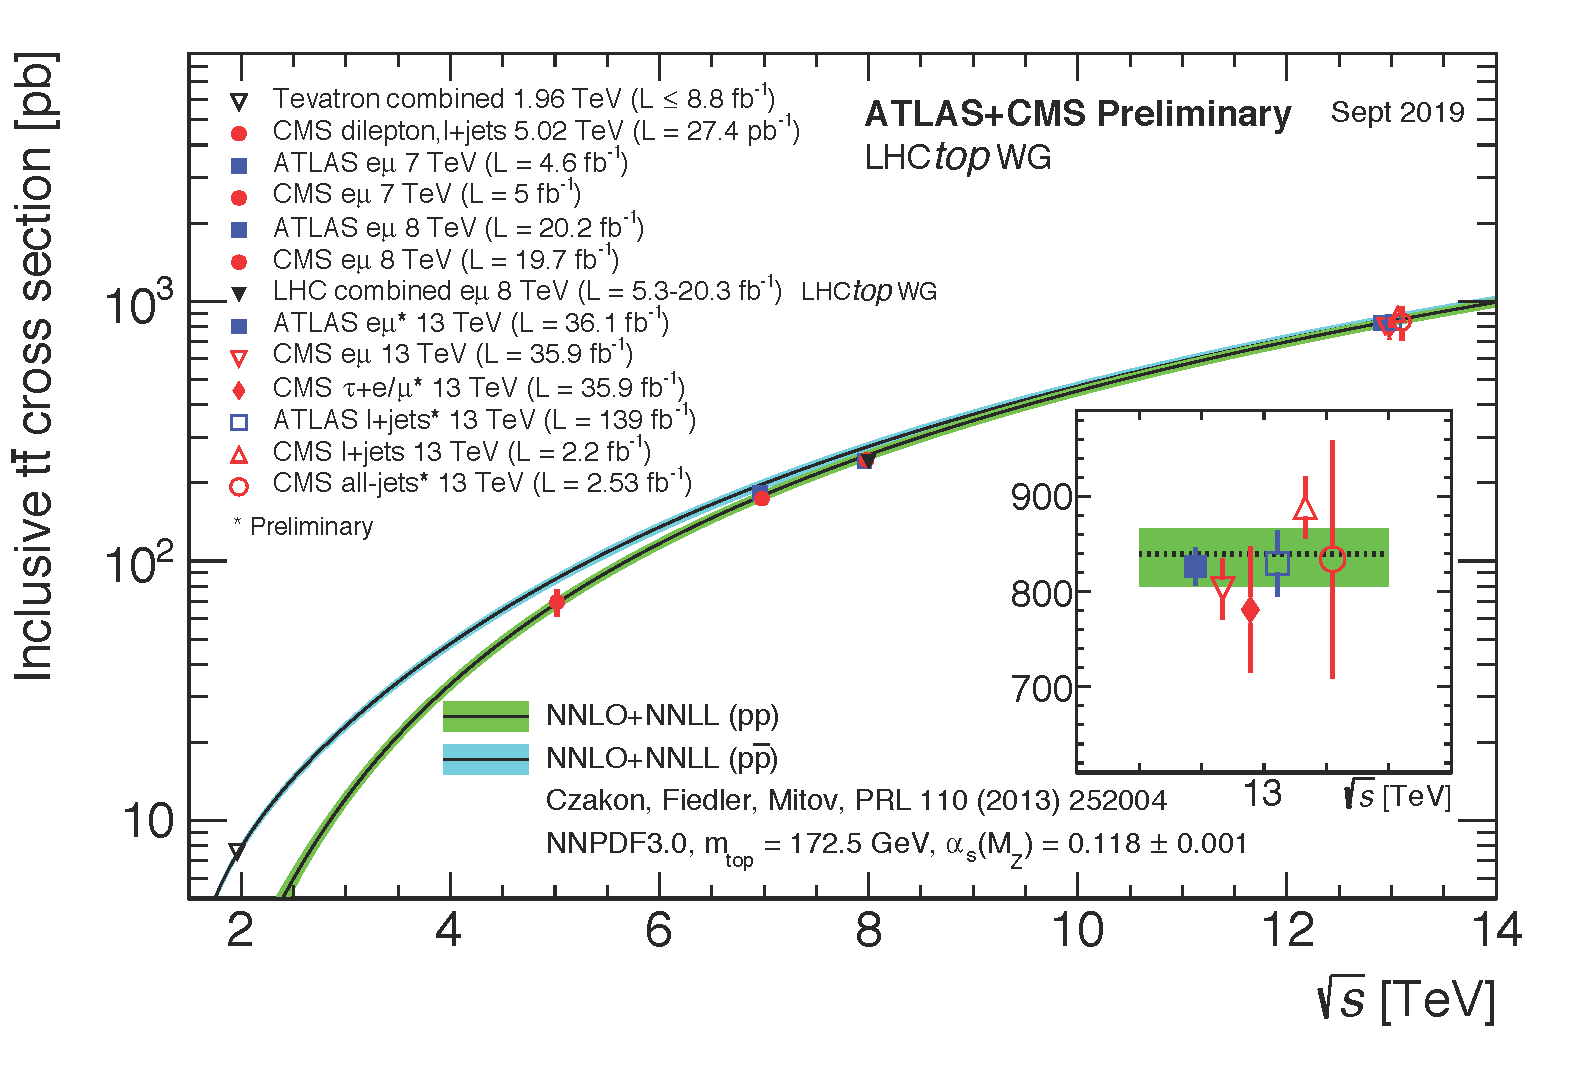
\includegraphics[height=0.7\textheight]{../../Thesis/ThesisImages/Theory/ttprodxsec.png}
	\captionof{figure}{$t\bar{t}$ production cross section \href{https://twiki.cern.ch/twiki/bin/view/LHCPhysics/LHCTopWGSummaryPlots}{[TopWGSummaryPlots]}}
}
\frame{\frametitle{Top Quark Decays}
\begin{columns}
\begin{column}{0.5\textwidth}
\begin{itemize}
\item Standard model top branching ratio to bW $\simeq 100\%$
\end{itemize}
\centering
 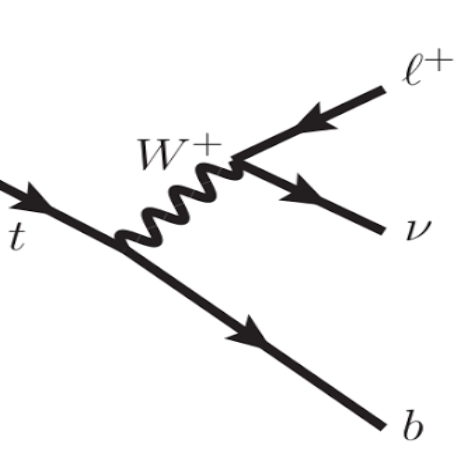
\includegraphics[width=0.7\textwidth]{../../Thesis/ThesisImages/topdecay.png}
 \captionof{figure}{Leptonic final state diagram for a top decay}
\end{column}
\begin{column}{0.5\textwidth}  %%<--- here
     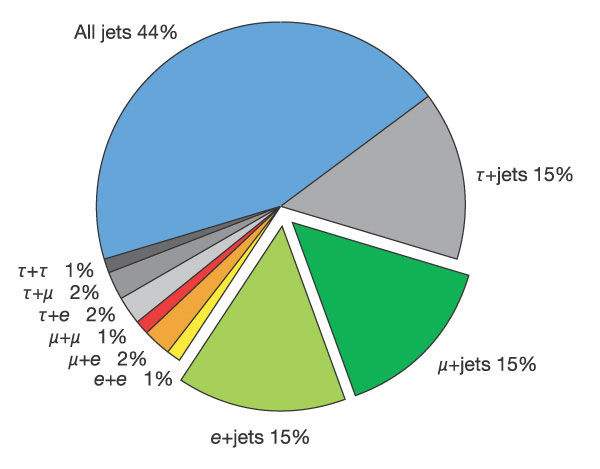
\includegraphics[width=1.1\textwidth]{../../Thesis/ThesisImages/Theory/topdecayproducts.jpg}
    \captionof{figure}{Top quark pair decay final states \href{https://images.nature.com/full/nature-assets/nature/journal/v429/n6992/images/nature02589-f2.2.jpg}{[Nature]}}
\end{column}
\end{columns}
}

\frame{\frametitle{Top Quark Decays in the SM}
\centering
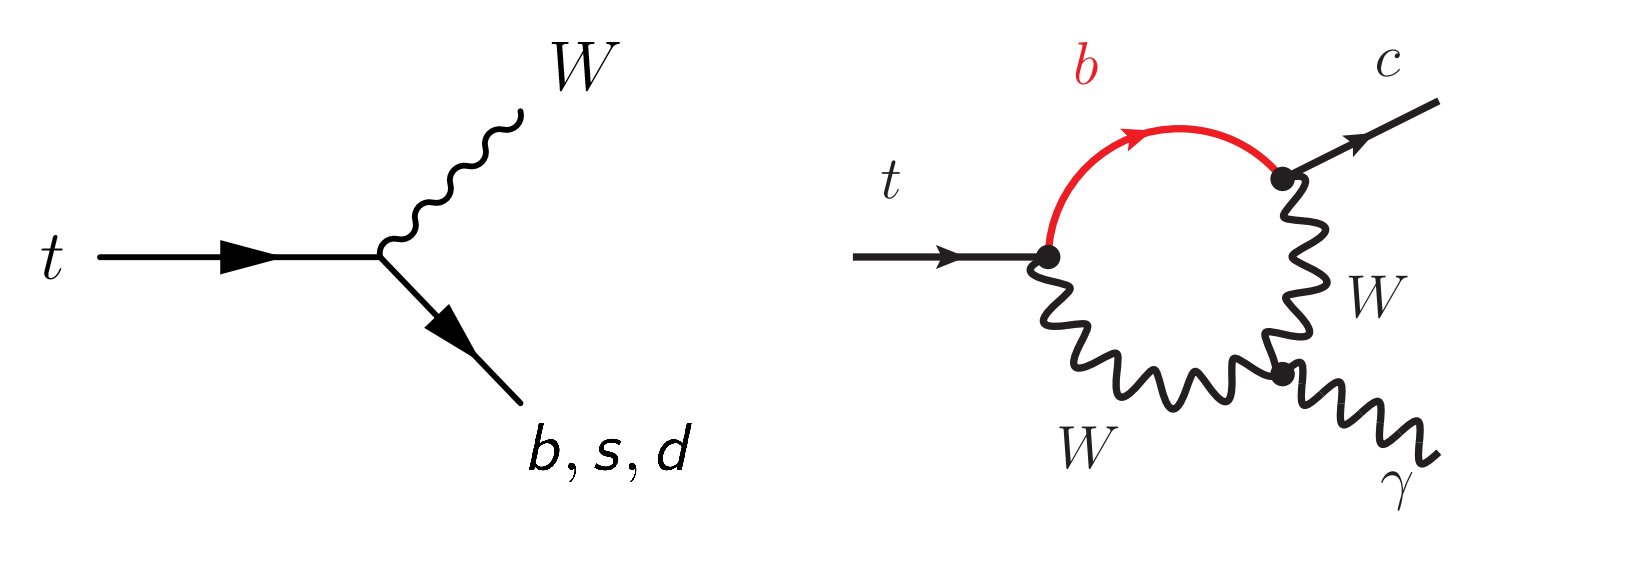
\includegraphics[width=1.\textwidth]{../../Thesis/ThesisImages/Theory/SMTopDecays2.png}

\begin{columns}
\begin{column}{0.5\textwidth}
\begin{itemize}
\item $t\rightarrow b W \approx 99.83\%$
\item $t\rightarrow s W \approx 0.16\%$
\item $t\rightarrow d W \approx 0.01\%$
\end{itemize}
\end{column}
\begin{column}{0.5\textwidth}
\begin{itemize}
\item $t\rightarrow q_{u,c} X\approx 10^{-17} - 10^{-12}$
\item Limits on $t\rightarrow \gamma q$ processes: \href{http://inspirehep.net/record/1750600?ln=en}{[Phys.Lett. B800 135082]}
	\begin{itemize}
	\item $t\rightarrow \gamma u < 2.8 x10^{-5}$
	\item $t\rightarrow \gamma c <  18 x 10^{-5}$
	\end{itemize}
\end{itemize}
\end{column}
\end{columns}
}


\subsection{Historical Background}
\frame{\frametitle{GIM Mechanism}
\begin{itemize}
\item Cabibbo model - 3 quarks (u, d, s)
\item Studies of kaon decays showed the existence of $K^+ \rightarrow \mu^+ \nu_\mu$ but an absence of predicted $K_{L}^0 \rightarrow \mu^+ \mu^-$
\item Even in the absence of a tree level decay $K_{L}^0$ decay the box diagram would be possible through an exchange of W bosons
\item Weak neutral current interactions in the uds model  have the form
\[
u\bar{u}+ (d\bar{d}\cos^2\theta_C+s\bar{s}\sin^2\theta_C)) +(s\bar{d} + d\bar{s})sin\theta_C cos\theta_C
\]
\end{itemize}
\centering
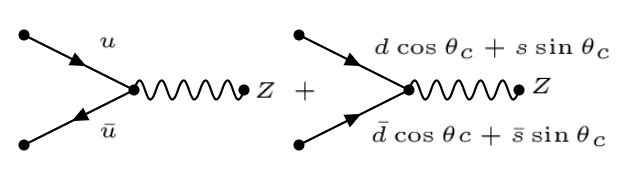
\includegraphics[width=0.45\textwidth]{../../Thesis/ThesisImages/gimdeltaSa.png}
}

\frame{\frametitle{GIM Mechanism}
\centering
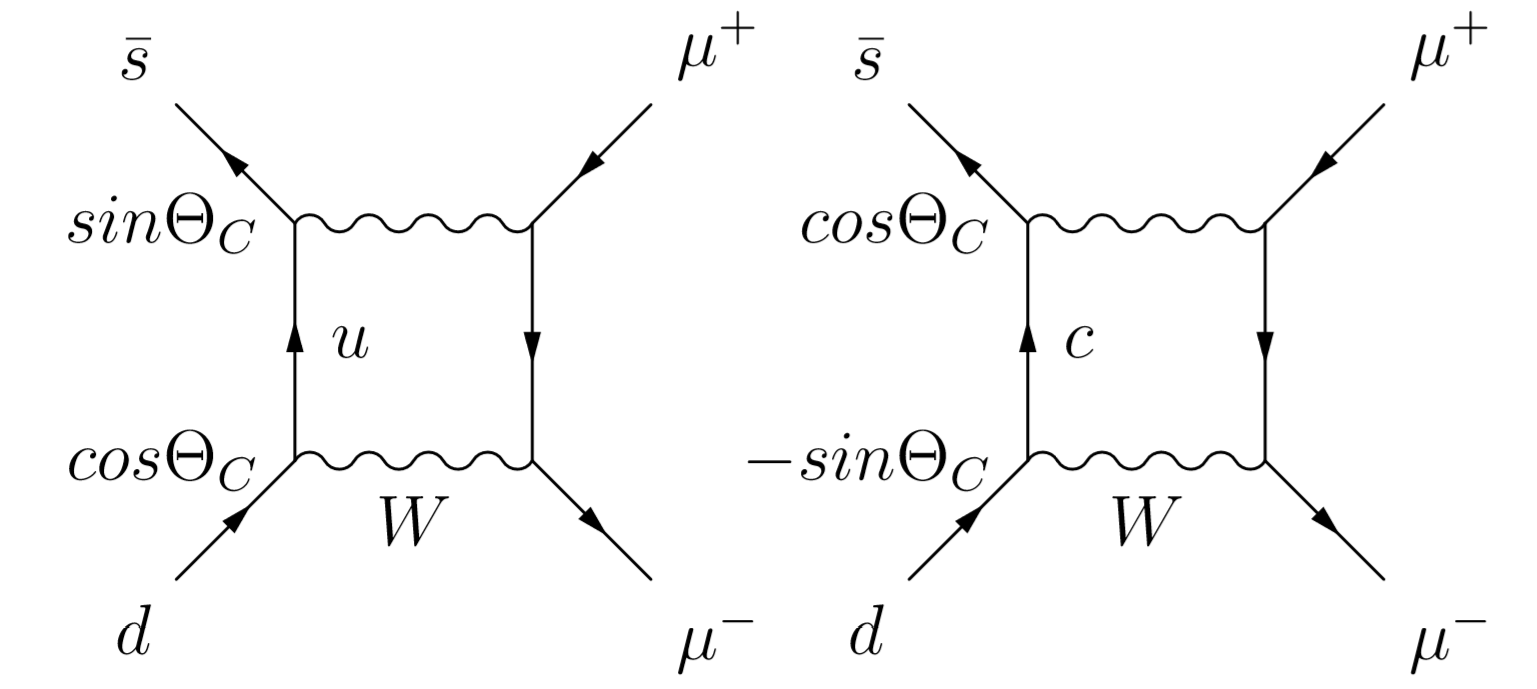
\includegraphics[width=.6\textwidth]{../../Thesis/ThesisImages/Theory/GIMDiagrams.png}

\begin{itemize}
\item Glashow, Iliopoulos, and Maiani \href{https://journals.aps.org/prd/abstract/10.1103/PhysRevD.2.1285}{[Phys. Rev. D (1970)]} propose a machanism through which FCNCs are suppressed in loop diagrams
	\begin{itemize}
	\item Introduction of charm quark
	\end{itemize}
\item Kaon decays imply no neutral current/natural suppression of neutral current
\end{itemize}
}

\frame{\frametitle{GIM Mechanism}
\centering
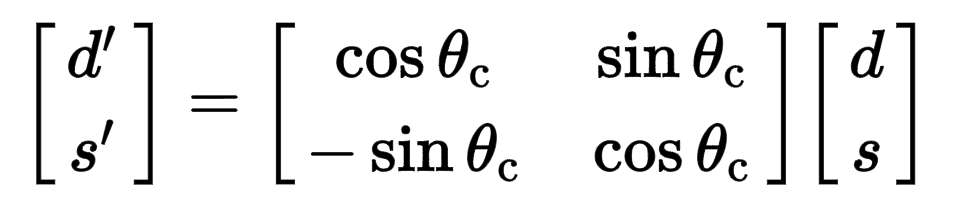
\includegraphics[width=.4\textwidth]{../../Thesis/ThesisImages/cabibboangle.png}
\begin{itemize}
\item The addition of the charm changes our weak neutral current interactions
\item With four quarks the weak neutral interactions now have the form:
\[
u\bar{u} + c\bar{c} + (d\bar{d}+s\bar{s}) \cos^2\theta_C + (s\bar{s} + d\bar{d})\sin^2\theta_C +(s\bar{d} + d\bar{s} - d\bar{s} - s\bar{d})sin\theta_C cos\theta_C
\]
\item Flavor changing neutral current diagrams cancel out at tree level (as $m_{c} \rightarrow m_{u}$)
\end{itemize}
\centering
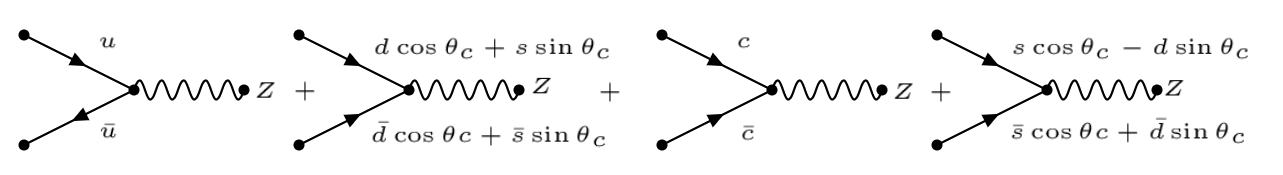
\includegraphics[width=0.9\textwidth]{../../Thesis/ThesisImages/Theory/gimdeltaS.png}
}


\frame{\frametitle{CKM Matrix}
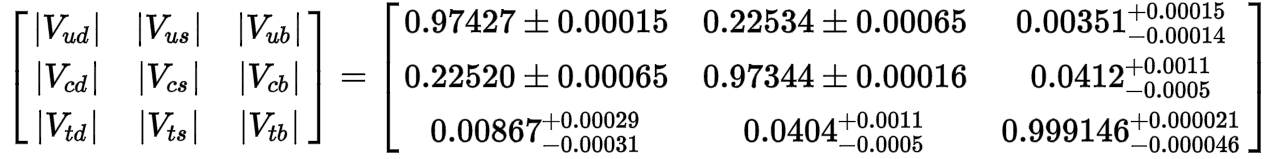
\includegraphics[width=1.\textwidth]{../../Thesis/ThesisImages/CKMMatrix.png}
\captionof{figure}{CKM Matrix}
\begin{itemize}
\item Decay rates proportional to $|V_{tX}|^2$
\item Top decay through a $W^{\pm}$ boson is a charged current interaction. 
\item Flavor changing processes are proportional to off-diagonal elements of the CKM matrix
\item GIM/CKM suppression of these FCNC processes in the Standard Model make them unlikely to be seen without some new physics
\end{itemize}
}
\subsection{Current Limits} 
\frame{\frametitle{Top Flavor Changing Neutral Currents (FCNCs)}
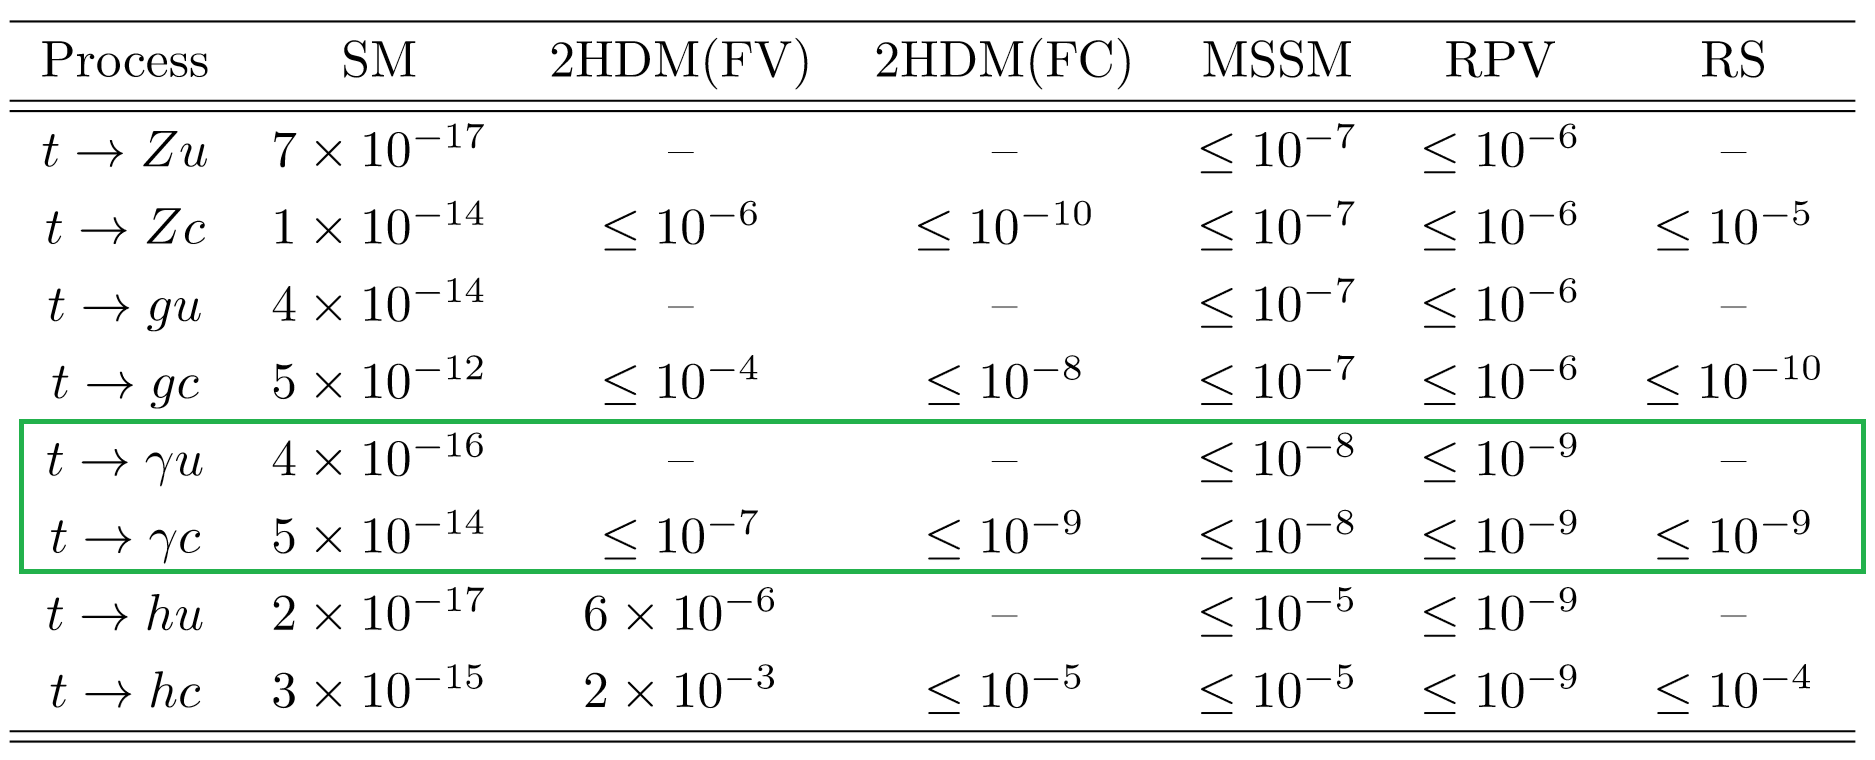
\includegraphics[width=1.\textwidth]{../../Thesis/ThesisImages/ModelLimits.png}
\captionof{table}{Branching ratio enhancements in various beyond the standard model theories \href{https://arxiv.org/pdf/1311.2028.pdf}{[Snowmass Top Report]}}

}

\frame{\frametitle{Top Flavor Changing Neutral Currents}
\begin{itemize}
\item Current Limits on FCNC Decays
\end{itemize}
\centering
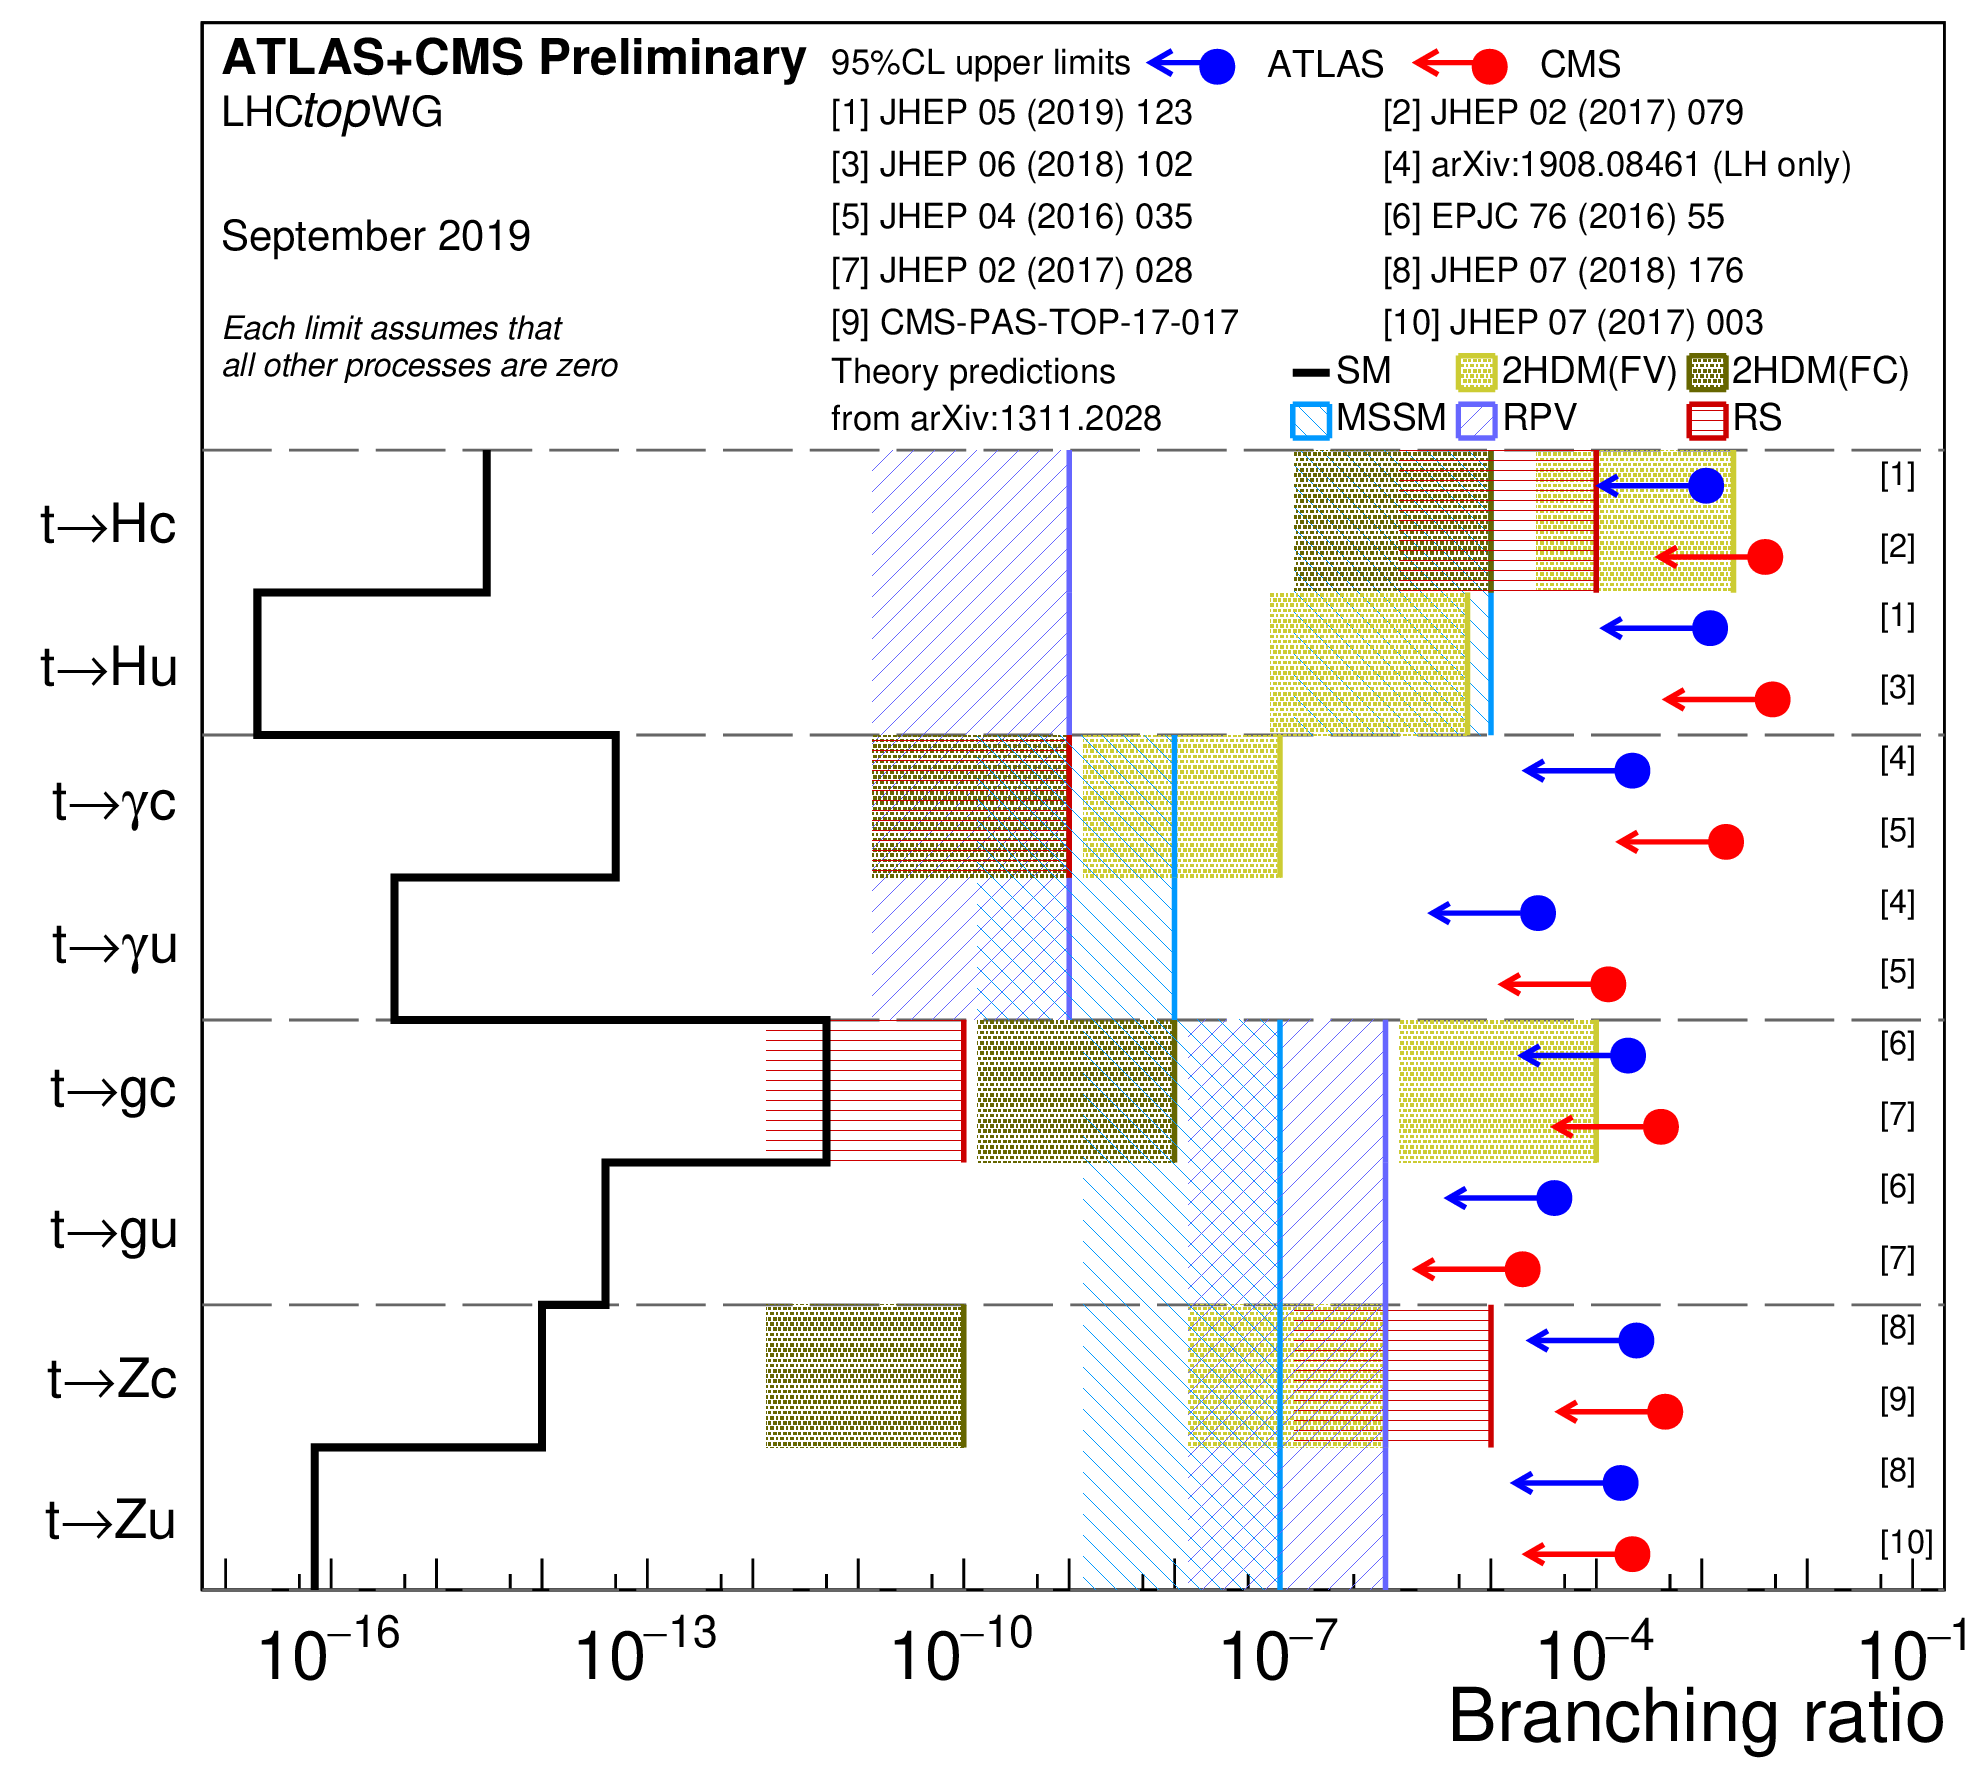
\includegraphics[width=0.55\textwidth]{../../Thesis/ThesisImages/Theory/AllFCNCLimits.png}
\begin{itemize}
\item Limits on $t\rightarrow q \gamma$ processes: \href{https://arxiv.org/abs/1511.03951}{[JHEP 04 (2016) 035]}
	\begin{itemize}
	\item $t\rightarrow \gamma u < 2.8 x10^{-5}$
	\item $t\rightarrow \gamma c <  18 x 10^{-5}$
	\end{itemize}
\end{itemize}
}

\frame{\frametitle{Monte Carlo Production of FCNC Signal Samples}
\begin{itemize}
\item Due to the low cross sections we must create our own Monte Carlo Samples for our Signal
\item An effective field theory approach was taken in the creation of the model [Degrande et al. Phys. Rev. D 91, 034024 (2015)]
\item This model takes advantage of dimension-6 operators
\end{itemize}
\[ \mathcal{L}_{SM} = \mathcal{L}_{SM}^{(4)} + \mathcal{L}^{eff} \text{ where } \mathcal{L}^{eff} = \frac{1}{\Lambda^2} \sum_{k} C_{k}^{(6)}Q_{k}^{(6)}
\]
\[ \mathcal{L}^{eff}_{tq\gamma} =  C \sigma^{\mu\nu}q_{\nu}(\lambda^{L}_{ct}P_L + \lambda^{R}_{ct}P_{R}) t A_{\mu} +H.c.
\]
}
\frame{\frametitle{FCNC: What are we looking for? $t\bar{t}\rightarrow W (\rightarrow l \nu) b+ q\gamma$}
\begin{itemize}
\item Final state topology
	\begin{itemize}
	\item One Neutrino, from W
	\item One Lepton, from W
	\item One B-jet, SM Top
	\item One Photon, FCNC Top
	\item One Jet, FCNC Top
	\end{itemize}
\end{itemize}
\centering
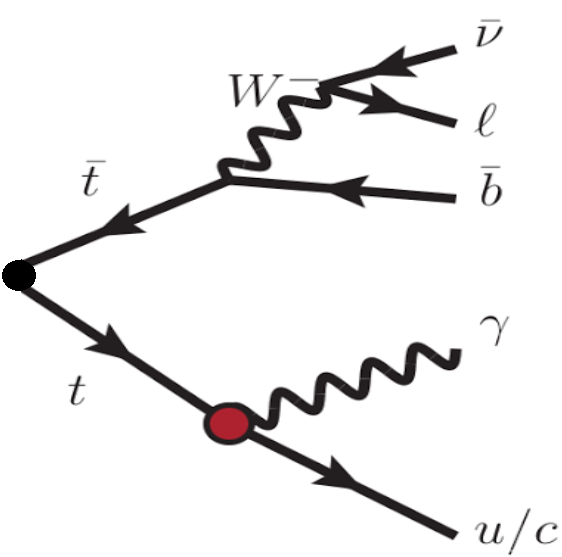
\includegraphics[width=0.3\textwidth]{../../Thesis/ThesisImages/fcncttbar.png}
}

\section{The LHC and ATLAS}
\subsection{The Large Hadron Detector}

\frame{\frametitle{The Large Hadron Collider}
\centering
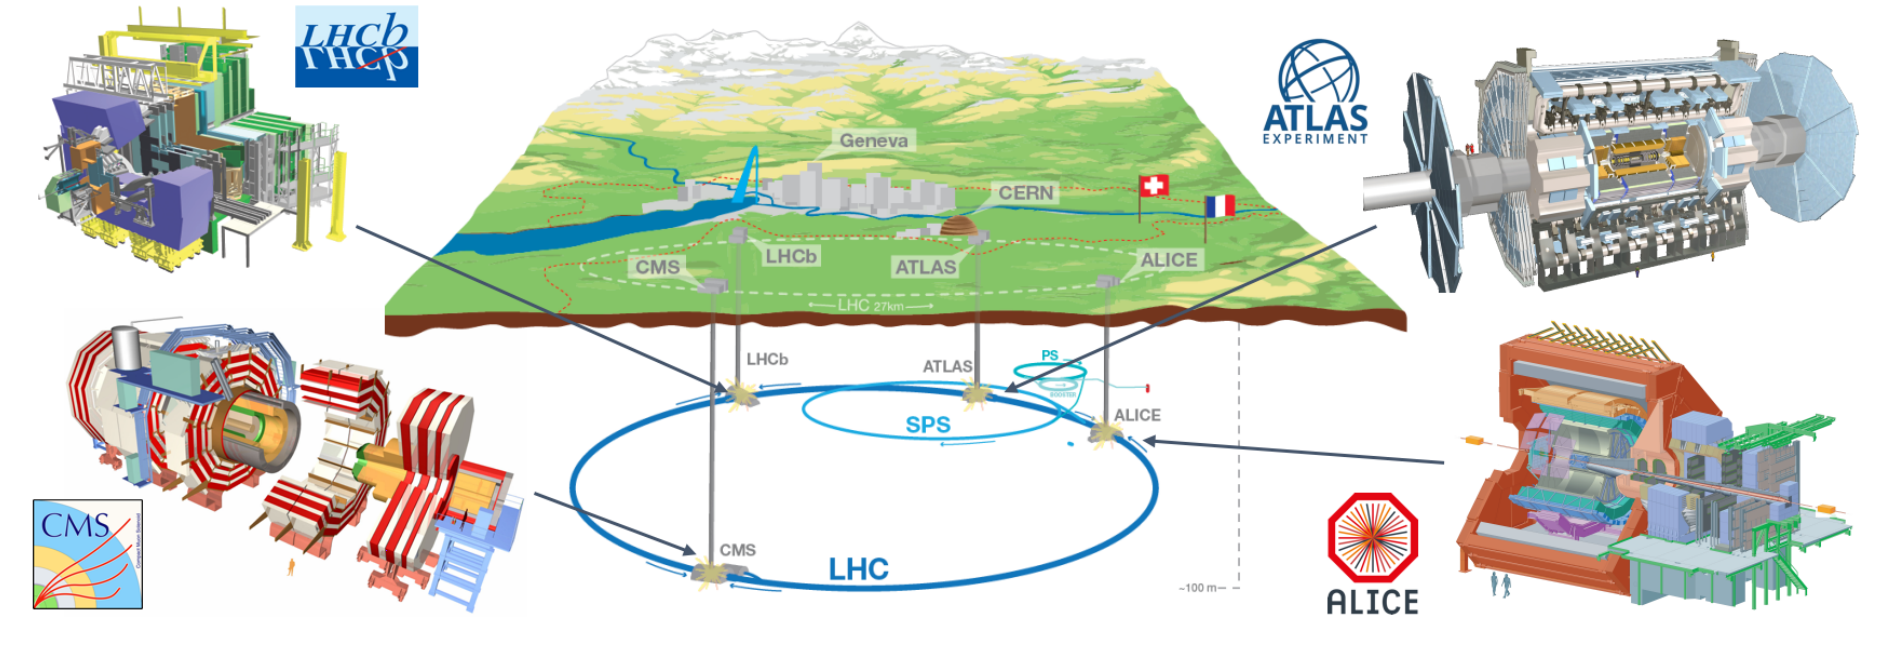
\includegraphics[width=\textwidth]{../../Thesis/ThesisImages/LHCImages/LHCDetecPlacement.png}
\begin{itemize}
\item 27km ring beneath Franco-Swiss border

\item Collides protons at center of mass energy 13TeV
\item Over 10 Quadrillion ($10^{15}$) events produced within the ATLAS detector so far
\end{itemize}
}

\subsection{The ATLAS Detector}
\frame{\frametitle{The ATLAS Detector}
\centering
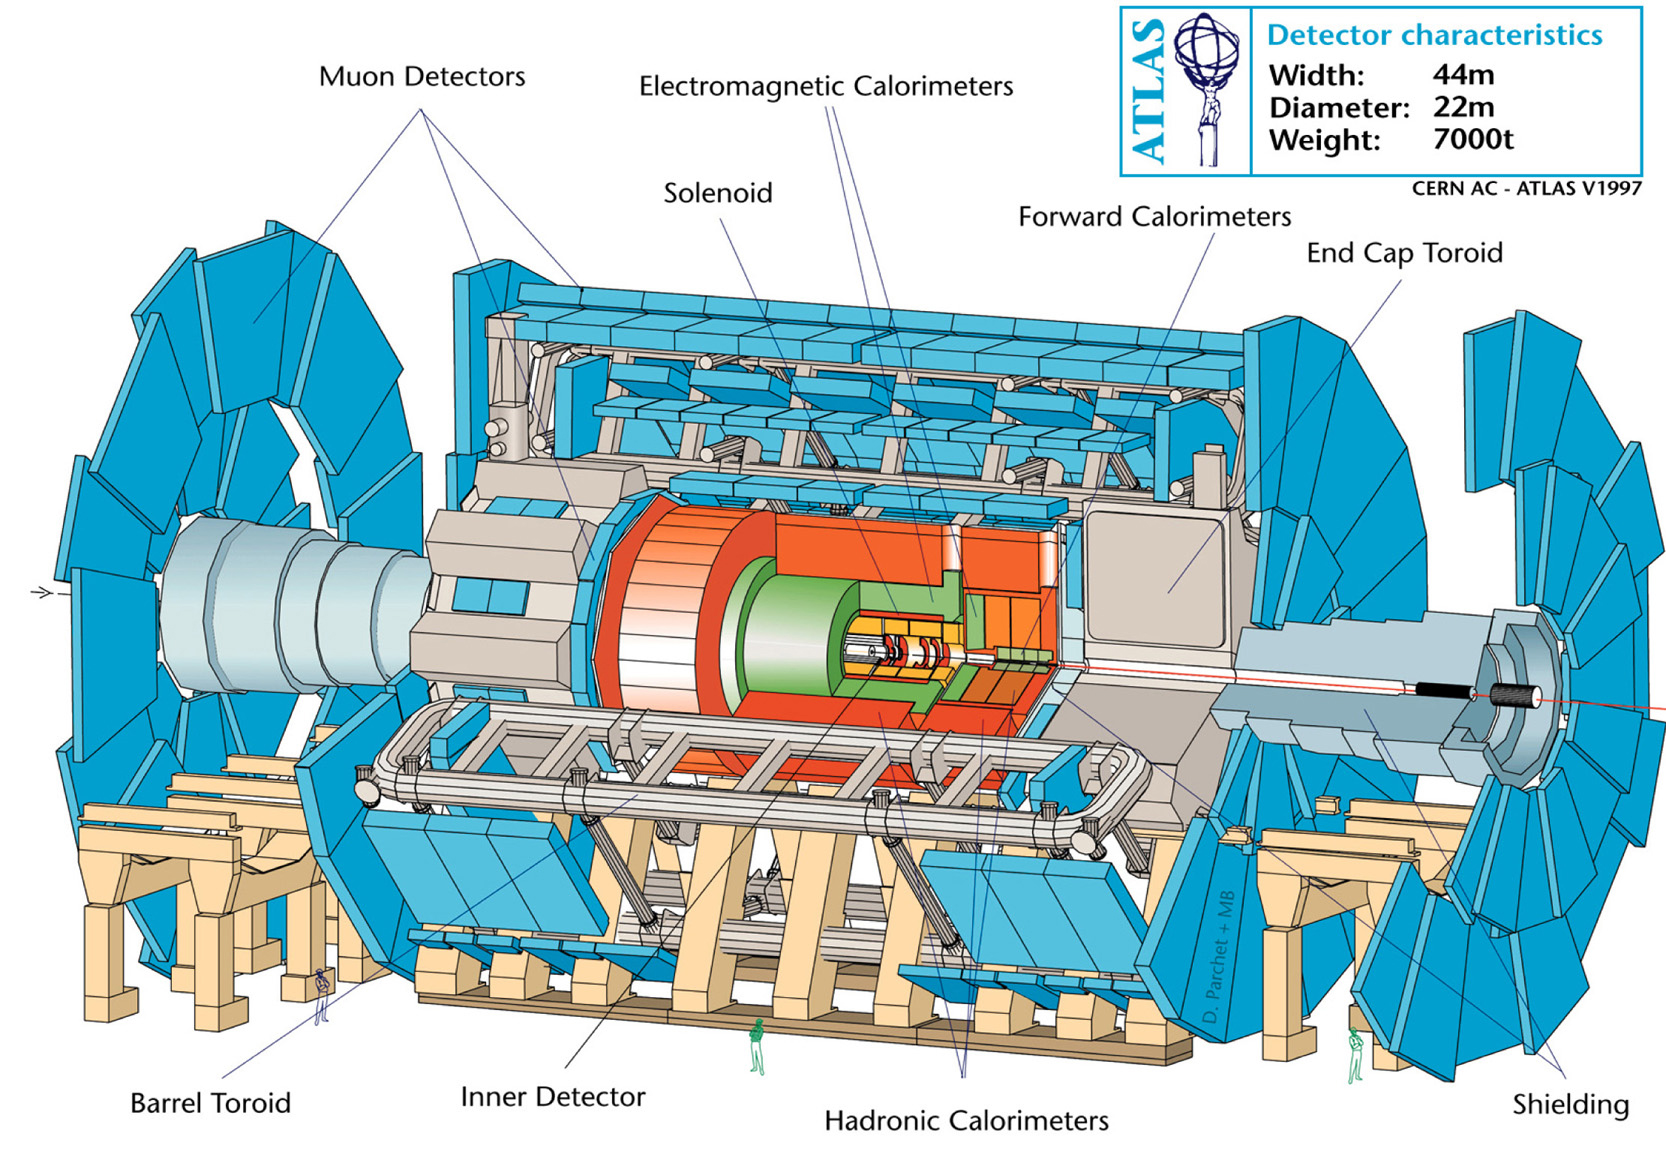
\includegraphics[width=.9\textwidth]{../../Thesis/ThesisImages/LHCImages/atlasdet.jpg}
}

\frame{\frametitle{Particles in ATLAS}
\centering 
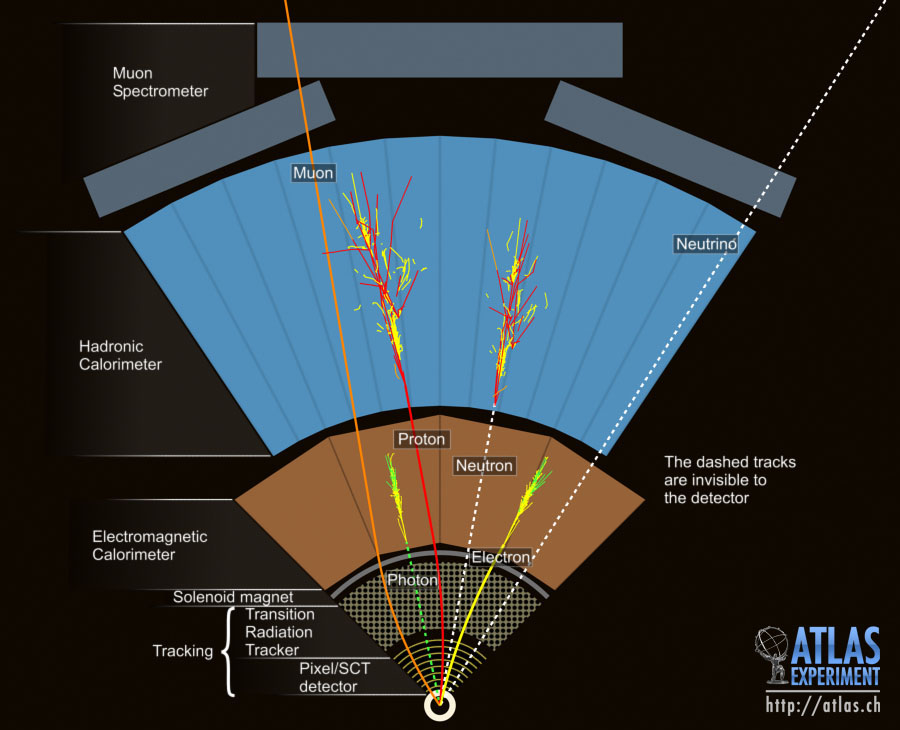
\includegraphics[width=.8\textwidth]{../../Thesis/ThesisImages/Simulation/ParticleInteractions.jpg}
}

\frame{\frametitle{ATLAS Data}
\begin{columns}
\begin{column}{0.6\textwidth}
\centering 
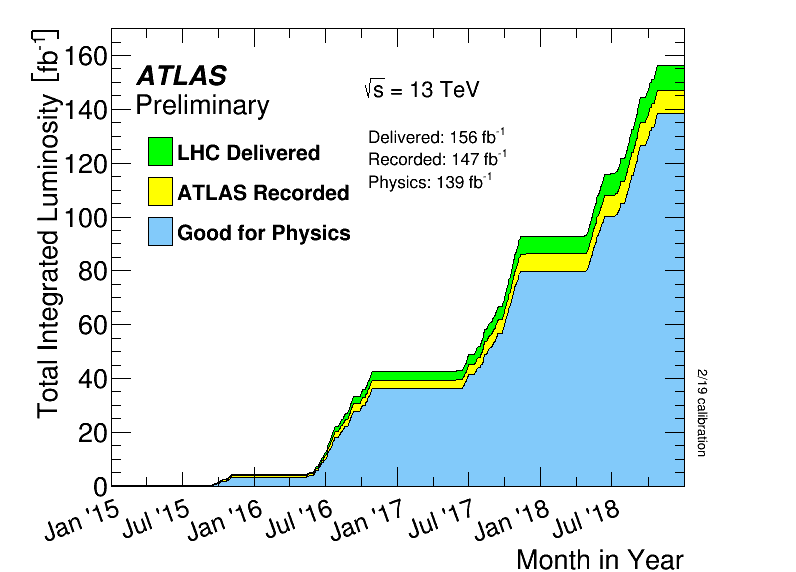
\includegraphics[width=.8\textwidth]{../../Thesis/ThesisImages/LHCImages/ATLASLumi.png}
\begin{itemize}
\item Total Luminosity at $\sqrt{s} = 13TeV$:  $139 \text{fb}^{-1}$
\item The number of events we see is $N=\sigma L$
\item $N_{tot} \approx 14x10^{15}$ events produced during the 13TeV data runs
\item $N_{t\bar{t}} \approx 116x10^6$
\end{itemize}
\end{column}
\begin{column}{0.5\textwidth}
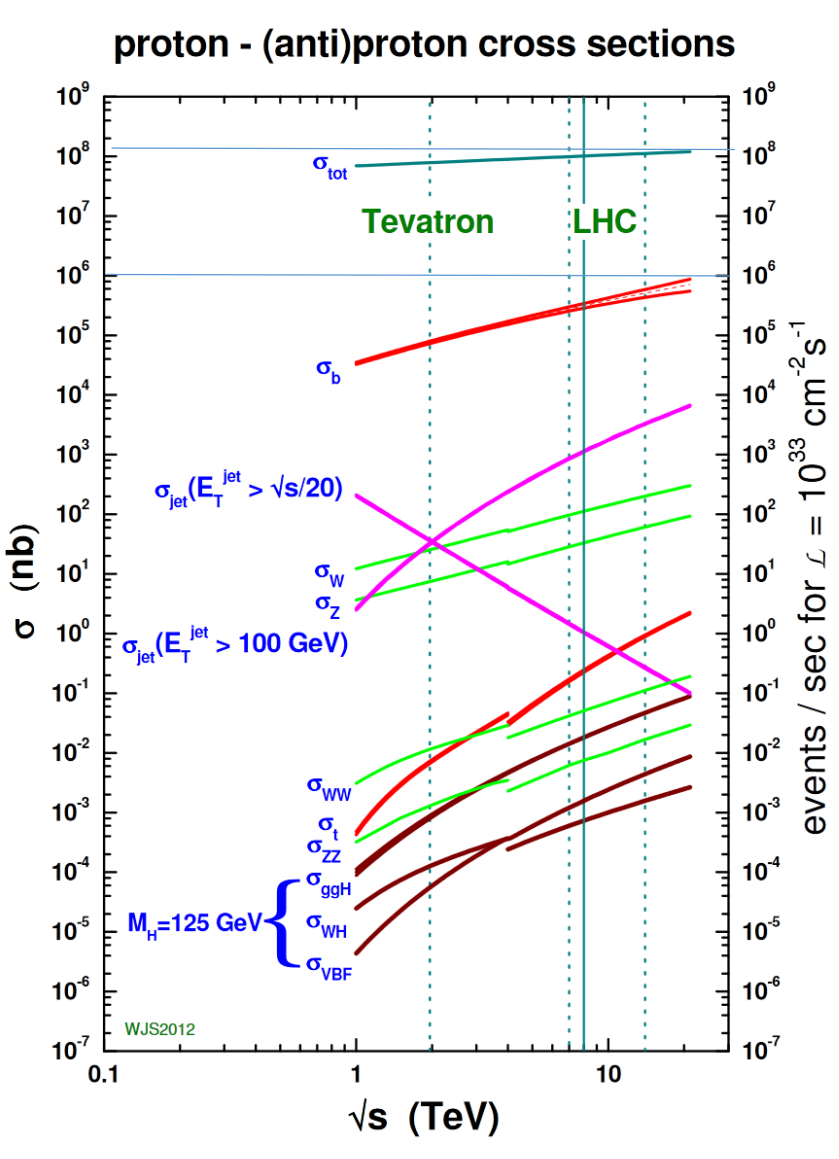
\includegraphics[width=.9\textwidth]{../../Thesis/ThesisImages/HardScatCrosSecs.png}
\end{column}
\end{columns}
}

%\frame{\frametitle{Events in ATLAS}
%\begin{columns}
%\begin{column}{0.5\textwidth}
%\centering
%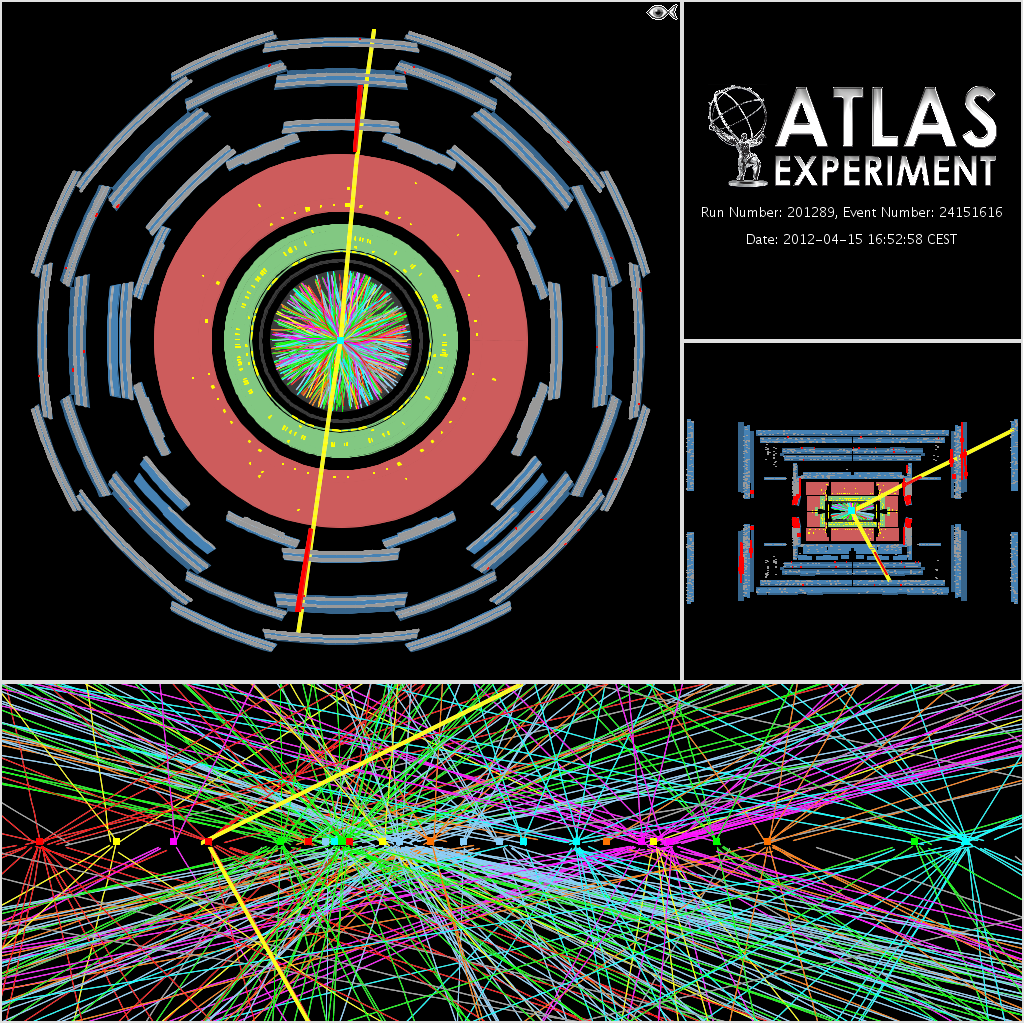
\includegraphics[width=\textwidth]{../../Thesis/ThesisImages/LHCImages/2012_highPileup.png}
%\end{column}
%\begin{column}{0.5\textwidth}
%\begin{itemize}
%\item LHC provides around 600 million interactions/second
%\item Save compelling events $\rightarrow$ 10s of PB/year
%\item Extremely large, messy data sets
%\item Detector well modeled with \textsc{Geant4} 
%\item Monte Carlo techniques used for background event generation
%\end{itemize}
%\end{column}
%\end{columns}
%}



\frame{\frametitle{ATLAS Data Acquisition}
\begin{columns}
\begin{column}{0.6\textwidth}
\begin{itemize}
\item Average 33.7 collisions per crossing during Run 2, 40MHz collision rate
\item Raw uncompressed event: 1.6 MB
\item Around 64 TB/s data
\item 2 Stage Trigger System
\begin{itemize}
\item Level 1 - Hardware based, coarse object reconstruction, reduces rate to under 100 kHz
\item High-Level Trigger: Software based, performs reconstruction as close to offline as possible, reduces rate to 1 kHz
\end{itemize}
\item Still save 10s of PB per year
\end{itemize}
\end{column}
\begin{column}{0.5\textwidth}
\centering 
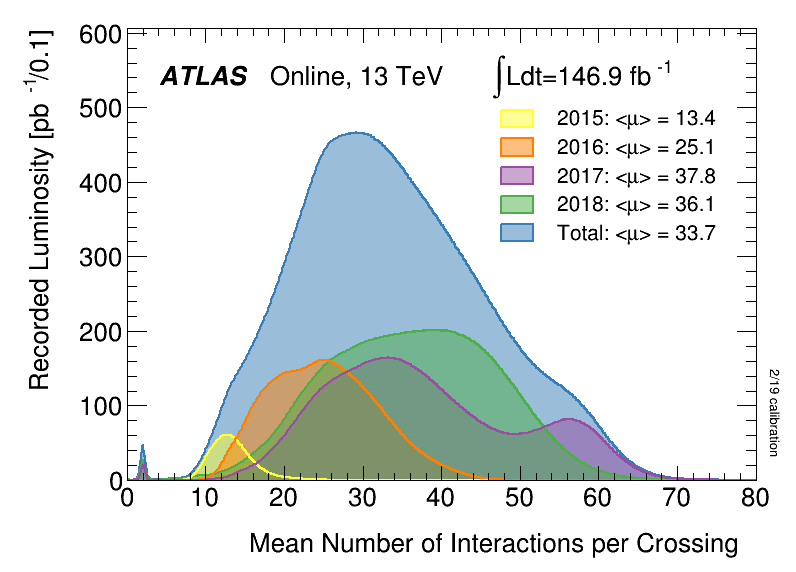
\includegraphics[width=.8\textwidth]{../../Thesis/ThesisImages/LHCImages/meanIntperCrossing.png}
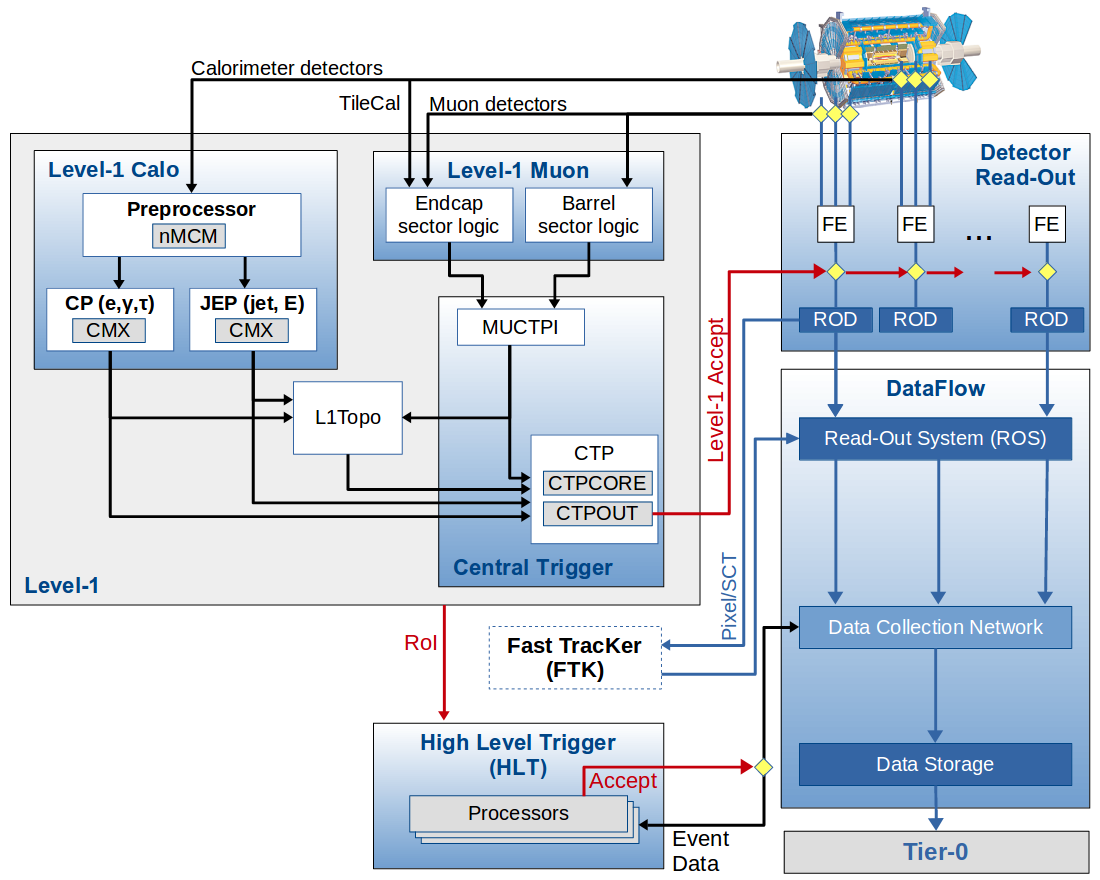
\includegraphics[width=.9\textwidth]{../../Thesis/ThesisImages/LHCImages/ATLASTDAQR2.png}
\end{column}
\end{columns}
}
%\frame{\frametitle{More ATLAS}
%}

\section{Searching for Flavor Changing Neutral Current Signatures}
\subsection{Object Selection}


\subsection{Region Creation}

\frame{\frametitle{Signal Region Preselection}
\begin{itemize}
\item Preselect events with objects that look like similar to our expected topology
\item Require:
	\begin{itemize}
	\item Exactly one lepton (e or $\mu$) $\geq$ 25 GeV
	\item Exactly one good photon $\geq$ 50GeV
	\item Missing transverse energy $\geq$ 30GeV
	\item $\geq 2$ jets (at least 1 b-tag)
	\end{itemize}
\end{itemize}
\centering
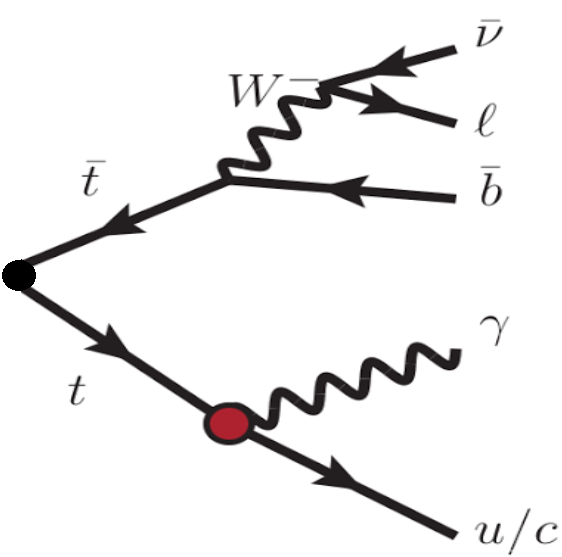
\includegraphics[width=0.3\textwidth]{../../Thesis/ThesisImages/fcncttbar.png}
}

\frame{\frametitle{Background Processes}
\begin{itemize}
\item Due to all of the processes at hadron colliders it is important to model similar event topologies well.
\item Major backgrounds include $t\bar{t}$, W+Jets, Z+Jets, + processes with an associated photon
\end{itemize}
\centering
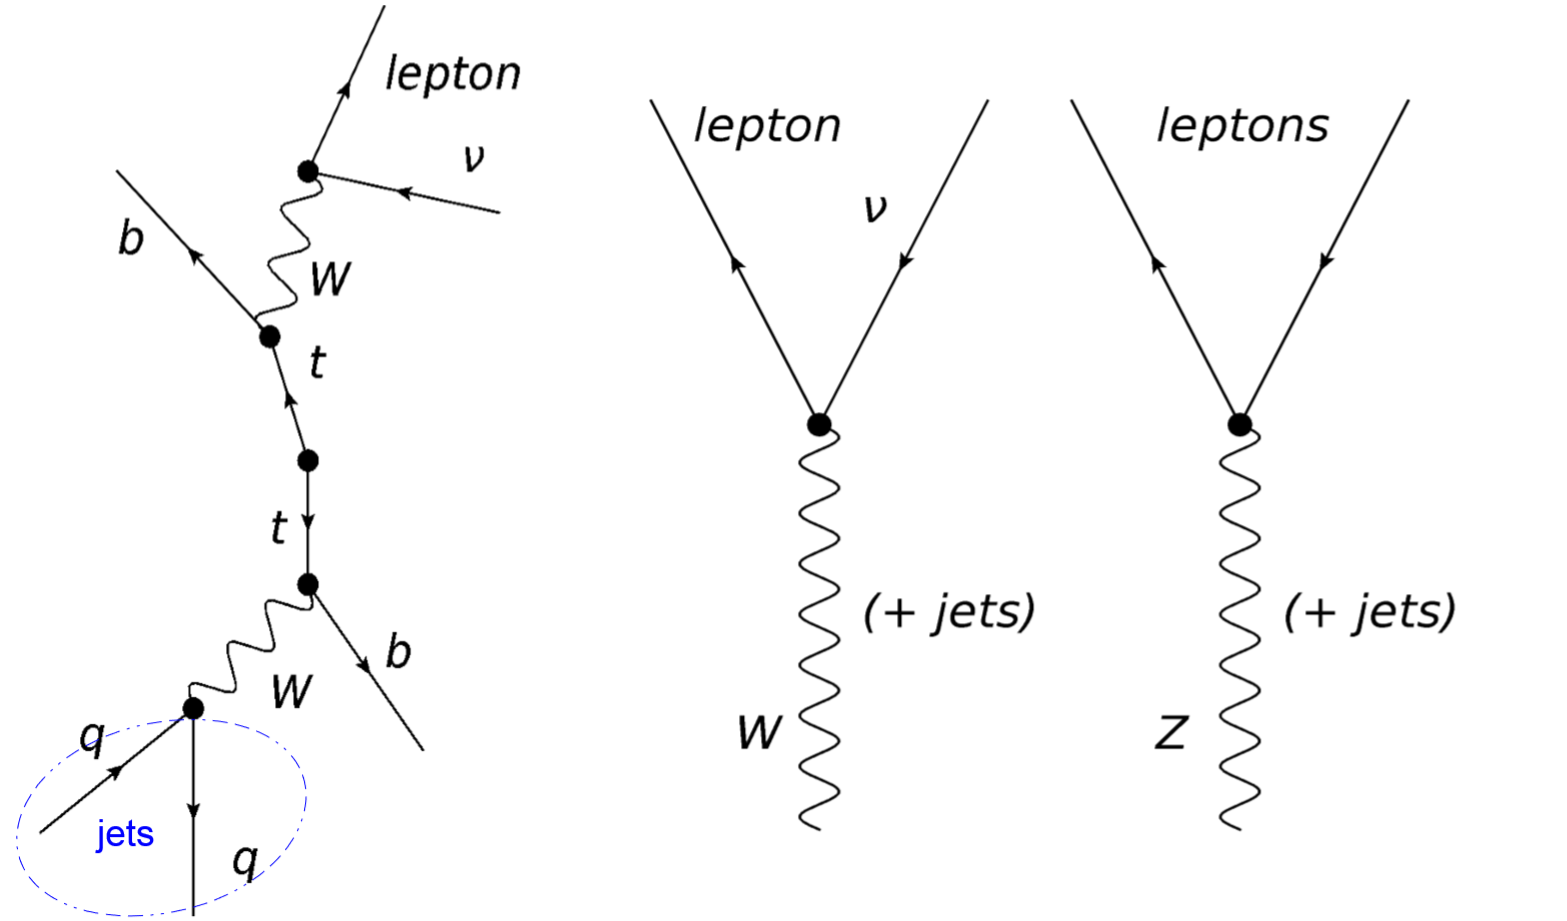
\includegraphics[width=0.6\textwidth]{../../Thesis/ThesisImages/backgrounds.png}
}


\frame{\frametitle{Preselection Objects}

\begin{columns}
\begin{column}{0.02\textwidth}

\rotatebox{90}{Muon Channel \qquad  Electron Channel} 
%\rotatebox{90}{Muon Channel        } 
\end{column}
\begin{column}{0.33\textwidth}
\begin{itemize}
\item  Leading Jet $p_T$
\end{itemize}
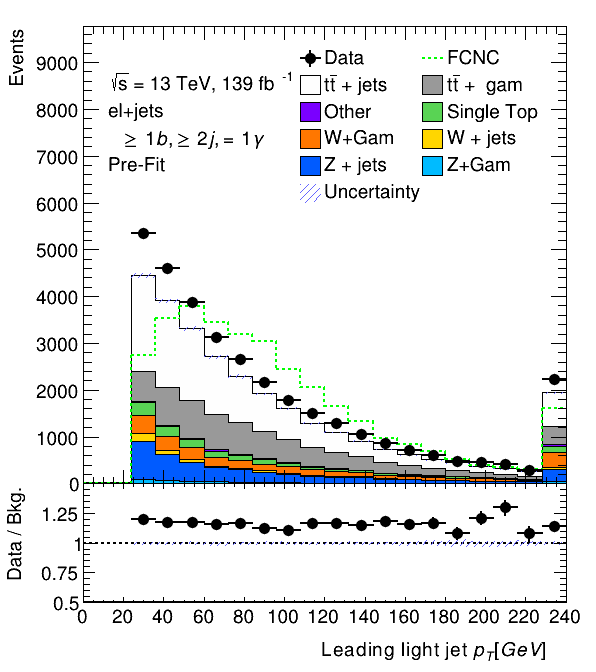
\includegraphics[width=.8\textwidth]{../../Thesis/ThesisImages/RegionPlots/BeforeScaling/PreSelection/FCNC_All_ejets/Plots/PreSel_jet0_pt.png} \\
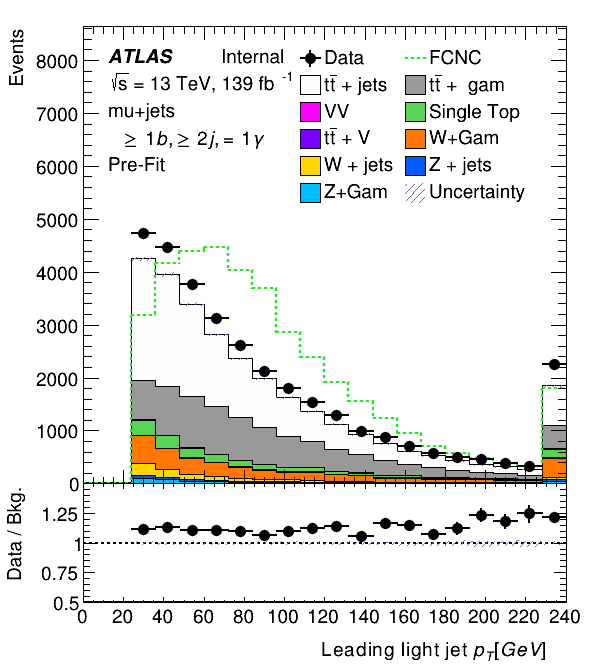
\includegraphics[width=.8\textwidth]{../../Thesis/ThesisImages/RegionPlots/BeforeScaling/PreSelection/FCNC_All_mujets/Plots/PreSel_jet0_pt.png}
\end{column}
\begin{column}{0.33\textwidth}
\begin{itemize}
\item Photon $p_T$
\end{itemize}
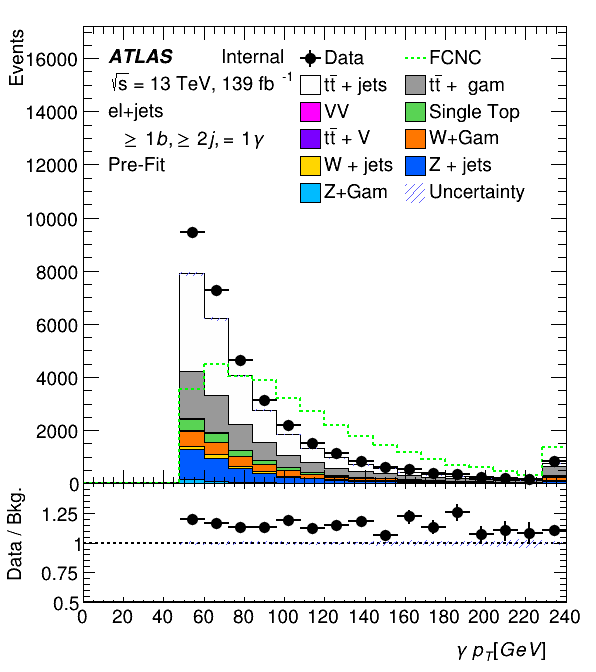
\includegraphics[width=.8\textwidth]{../../Thesis/ThesisImages/RegionPlots/BeforeScaling/PreSelection/FCNC_All_ejets/Plots/PreSel_ph_pt.png} \\
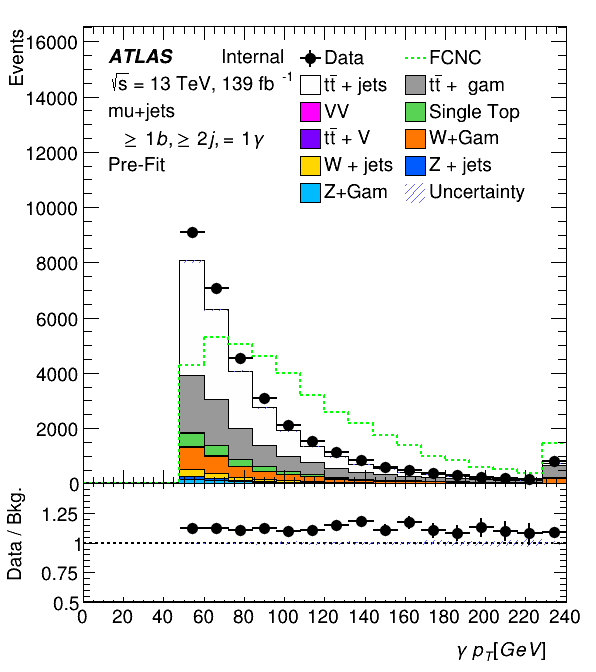
\includegraphics[width=.8\textwidth]{../../Thesis/ThesisImages/RegionPlots/BeforeScaling/PreSelection/FCNC_All_mujets/Plots/PreSel_ph_pt.png}
\end{column}
\begin{column}{0.33\textwidth}
\begin{itemize}
\item Lepton $p_T$
\end{itemize}
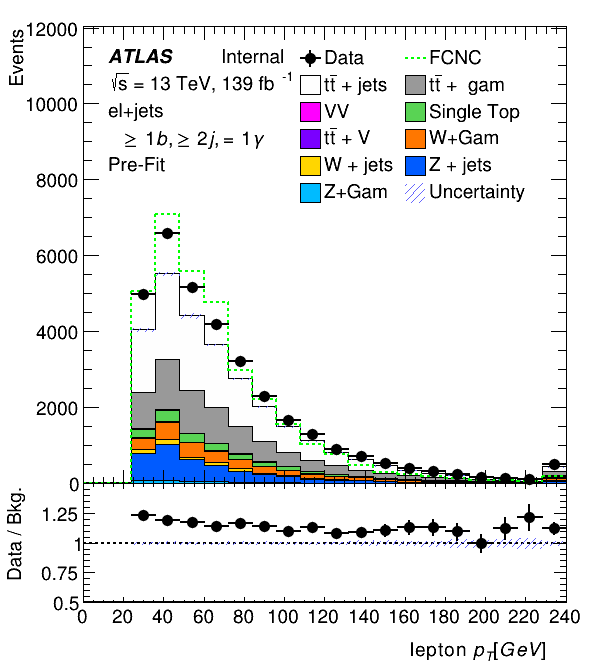
\includegraphics[width=.8\textwidth]{../../Thesis/ThesisImages/RegionPlots/BeforeScaling/PreSelection/FCNC_All_ejets/Plots/PreSel_lep_pt.png}\\
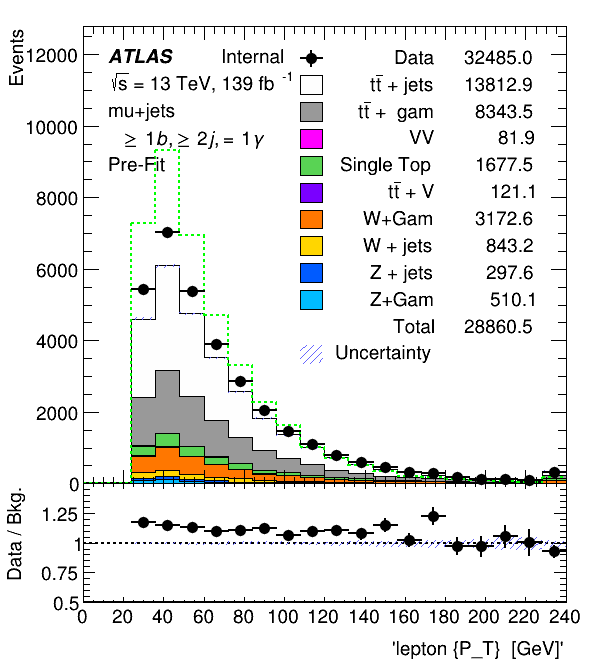
\includegraphics[width=.8\textwidth]{../../Thesis/ThesisImages/RegionPlots/BeforeScaling/PreSelection/FCNC_All_mujets/Plots/PreSel_lep_pt.png}
\end{column}
\end{columns}

}

\frame{\frametitle{Top Quarks}
Tops must be reconstructed from these basic physics objects along with b-jets and $E_{T}^\text{miss}$
\begin{itemize}
\item Neutrino z-axis direction is ambiguous, determined by minimization of: $\chi^2 = \frac{(m_{b,l,\nu}-m_t)^2}{\sigma^2_{SMtop}}+\frac{(m_{l,\nu}-m_W)^2}{\sigma^2_W} $
\end{itemize}
\begin{columns}
%\begin{column}{0.33\textwidth}
%\centering
%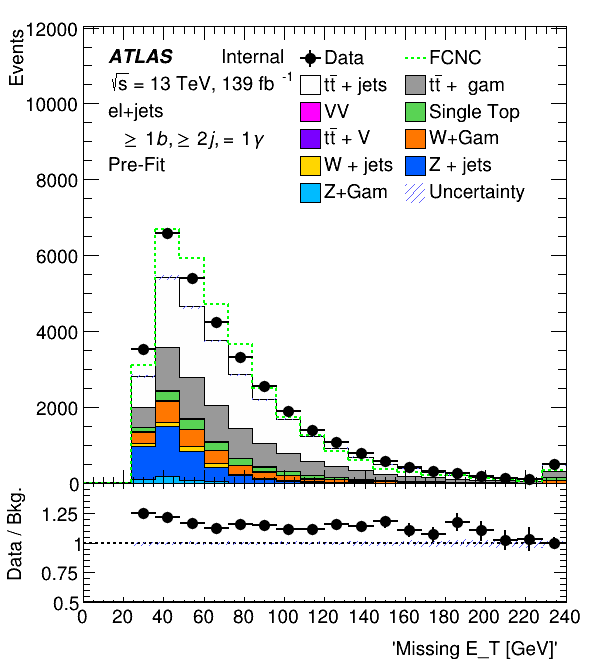
\includegraphics[width=.8\textwidth]{../../Thesis/ThesisImages/RegionPlots/BeforeScaling/PreSelection/FCNC_All_ejets/Plots/PreSel_met.png}\\
%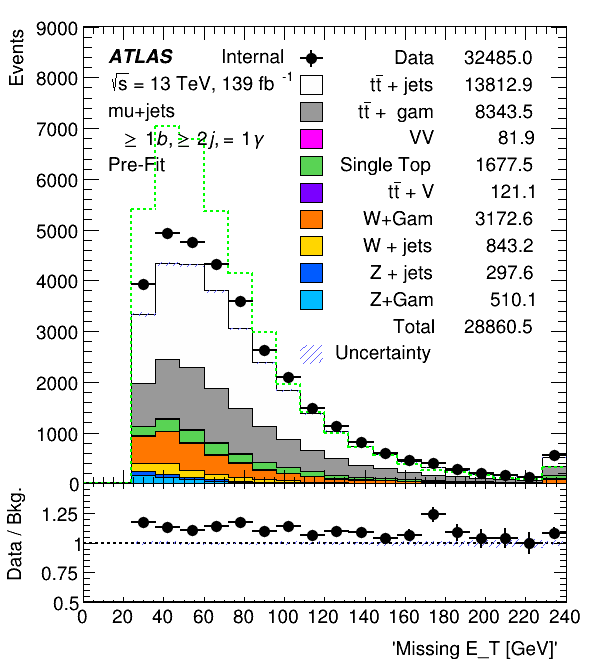
\includegraphics[width=.8\textwidth]{../../Thesis/ThesisImages/RegionPlots/BeforeScaling/PreSelection/FCNC_All_mujets/Plots/PreSel_met.png}
%\end{column} 
\begin{column}{0.55\textwidth}
SM Top: $m_{Wb}$\\
\centering
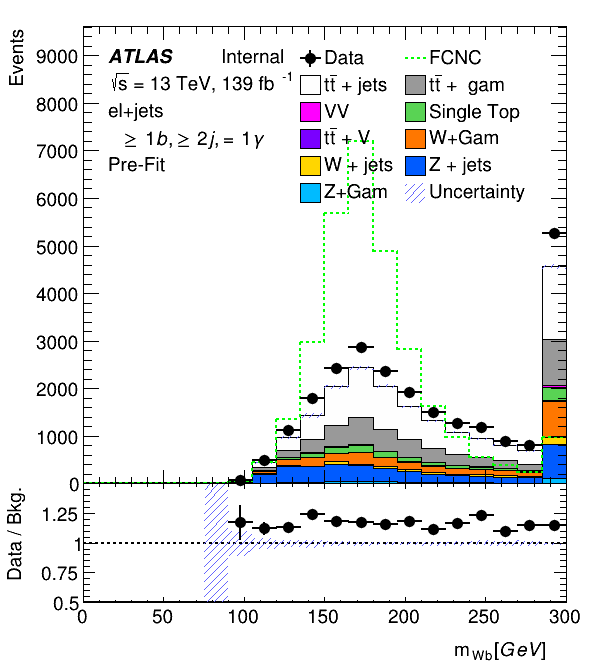
\includegraphics[width=.45\textwidth]{../../Thesis/ThesisImages/RegionPlots/BeforeScaling/PreSelection/FCNC_All_ejets/Plots/PreSel_SMtop.png}
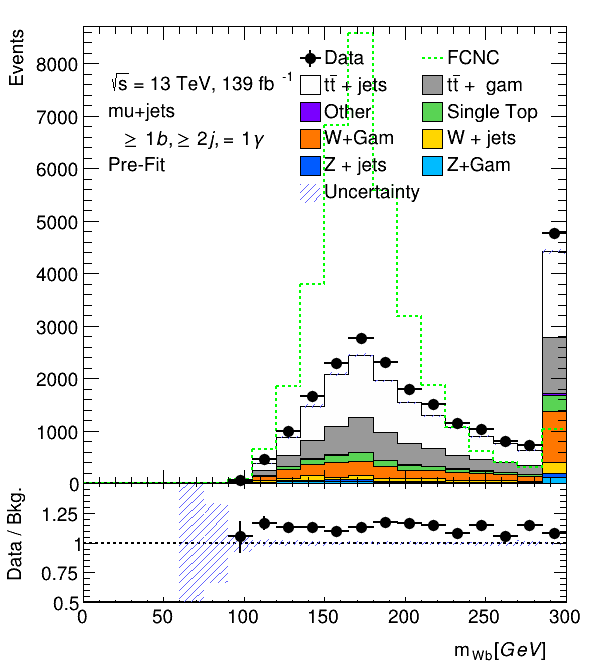
\includegraphics[width=.45\textwidth]{../../Thesis/ThesisImages/RegionPlots/BeforeScaling/PreSelection/FCNC_All_mujets/Plots/PreSel_SMtop.png}
\end{column}
\begin{column}{0.55\textwidth}
FCNC Top: $m_{q\gamma}$\\
\centering
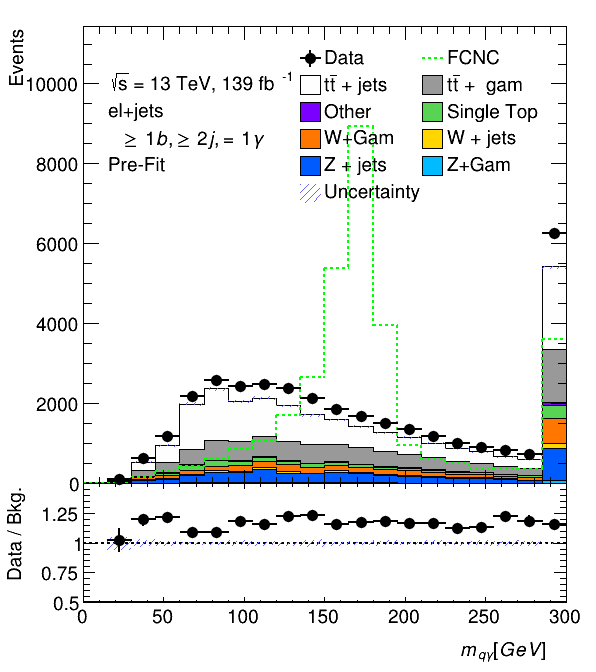
\includegraphics[width=.45\textwidth]{../../Thesis/ThesisImages/RegionPlots/BeforeScaling/PreSelection/FCNC_All_ejets/Plots/PreSel_mqph.png}
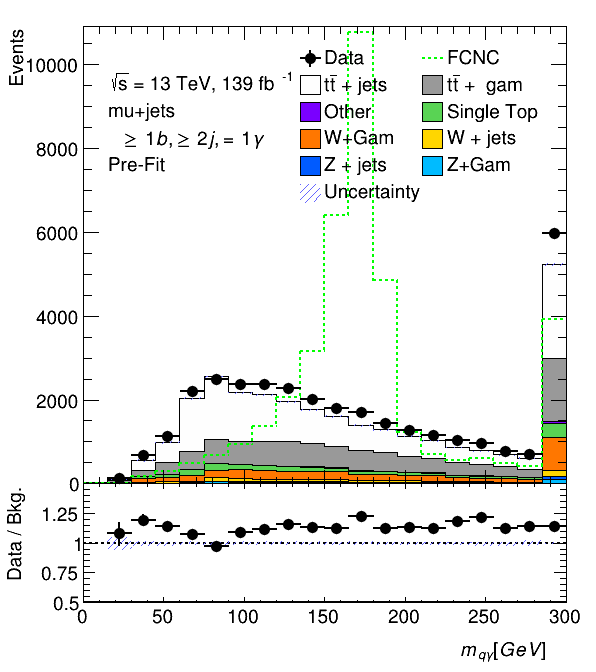
\includegraphics[width=.45\textwidth]{../../Thesis/ThesisImages/RegionPlots/BeforeScaling/PreSelection/FCNC_All_mujets/Plots/PreSel_mqph.png}
\end{column}
\end{columns}
}

\frame{\frametitle{Additional Processes}
\begin{itemize}
\item QCD Backgrounds are difficult to model at the energies and interaction rates of the LHC
\begin{itemize}
\item Develop 0 photon regions for scale factors for major backgrounds ($t\bar{t}$ and W+jets)
\end{itemize}
\item Photon misidentification i.e., particles being reconstructed as particles ($e\rightarrow \gamma$, $j\rightarrow \gamma$)
\begin{itemize}
\item $e\rightarrow \gamma$: $Z\rightarrow ee$ tag and probe method used for SF calculation
\item $j\rightarrow \gamma$: ABCD method used for SF calculation
\end{itemize}
\end{itemize}
}


\frame{\frametitle{0 Photon Backgrounds}

Select events with objects that look like similar to our expected topology for major backgrounds ($t\bar{t}$, W+jets)
Require:
\begin{itemize}
	\item Common Object Selection (MET,Triggers, etc.)
	\item Exactly one lepton (e or $\mu$) $\geq$ 25 GeV
	\item Number of Jets to define Regions:
	\begin{itemize}
	\item W+jets enriched region: $n_\text{jets}=3$
	\item Validation Region: $n_\text{jets}= 4$ 
	\item $t\bar{t}$+jets enriched region: $n_\text{jets}\geq 5$
	\end{itemize}
	\item Exactly 1 b-tagged jet
	\item $\geq 2$ jets (at least 1 b-tag)
\end{itemize}
Calculate scale factors simultaneously:
\[ 
\begin{bmatrix}  
N(W)_{3j} & N(t\bar{t})_{3j} \\ N(W)_{5+j} & N(t\bar{t})_{5+j} \end{bmatrix} \begin{bmatrix} W_{SF} \\ t\bar{t}_{SF} \end{bmatrix} =
 \begin{bmatrix} N(\text{data-bkg})_{3j} \\N(\text{data-bkg})_{5j} \end{bmatrix}
\]
\begin{table}[h]
\begin{center}
{\renewcommand{\arraystretch}{1.2}
\begin{tabular}{ccc}
\hline
Sample     &  e+jets SF   & $\mu$+jets SF  \\  \hline 
W+jets    &  1.22   &  1.25	\\
$t\bar{t}$  &  1.06    &  1.01	\\ \hline
\end{tabular}
}
\end{center}
\end{table}
}
\frame{\frametitle{0 Photon Scale Factors, $m_{Wb}$ distributions before SF}
\begin{columns}
\begin{column}{0.02\textwidth}
\rotatebox{90}{Muon Channel \qquad  Electron Channel} 
%\rotatebox{90}{Muon Channel        } 
\end{column}
\begin{column}{0.33\textwidth}
\begin{itemize}
\item  W+jets Enriched
\end{itemize}
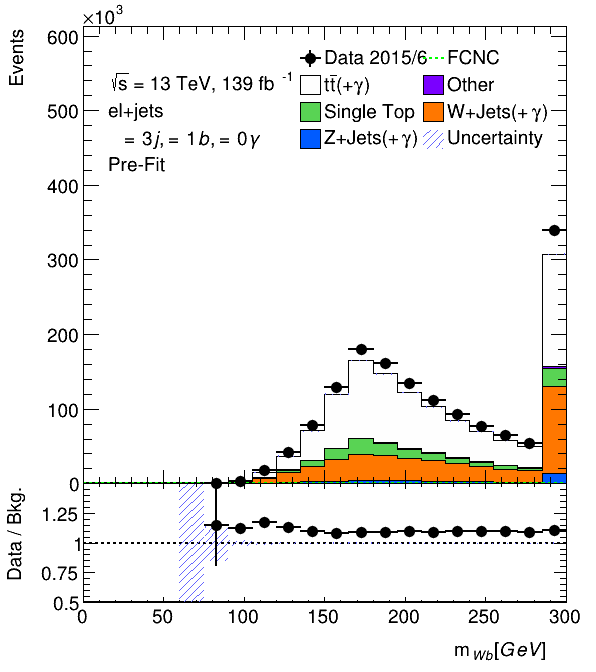
\includegraphics[width=.8\textwidth]{../../Thesis/ThesisImages/RegionPlots/AfterScaling/ControlRegions/HardCodedNormFactor/FCNC_All_ejets/Plots/CR1_SMtop.png} \\
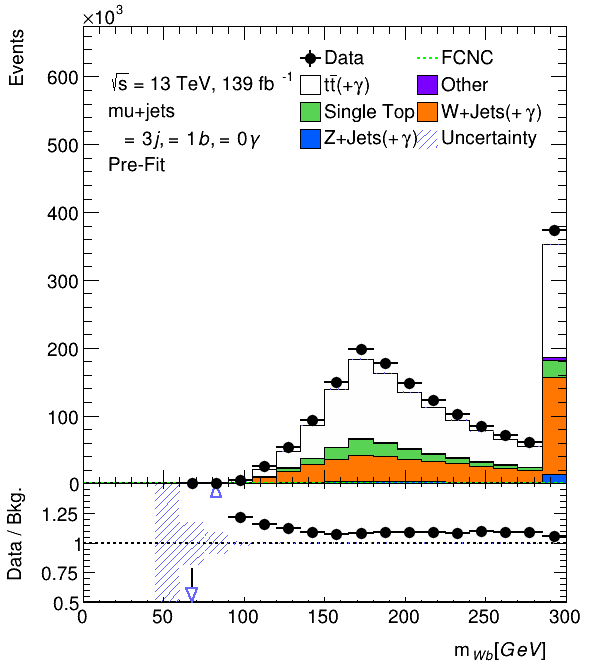
\includegraphics[width=.8\textwidth]{../../Thesis/ThesisImages/RegionPlots/AfterScaling/ControlRegions/HardCodedNormFactor/FCNC_All_mujets/Plots/CR1_SMtop.png}
\end{column}
\begin{column}{0.33\textwidth}
\begin{itemize}
\item $t\bar{t}$ Enriched
\end{itemize}
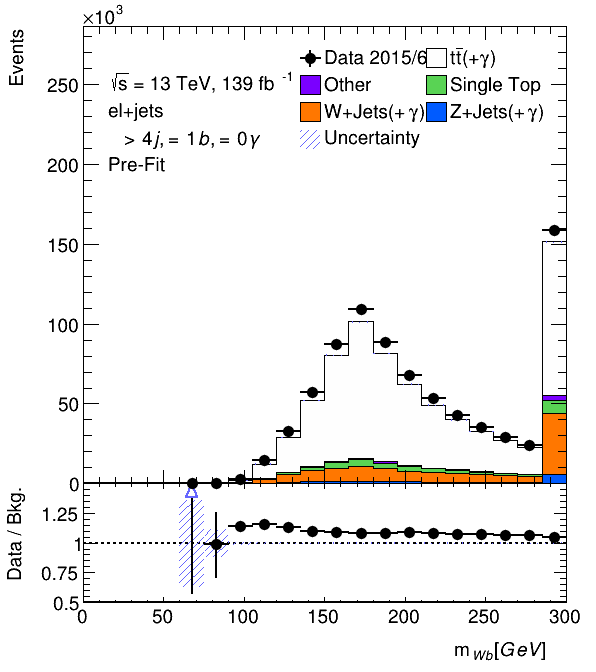
\includegraphics[width=.8\textwidth]{../../Thesis/ThesisImages/RegionPlots/AfterScaling/ControlRegions/HardCodedNormFactor/FCNC_All_ejets/Plots/CR2_SMtop.png} \\
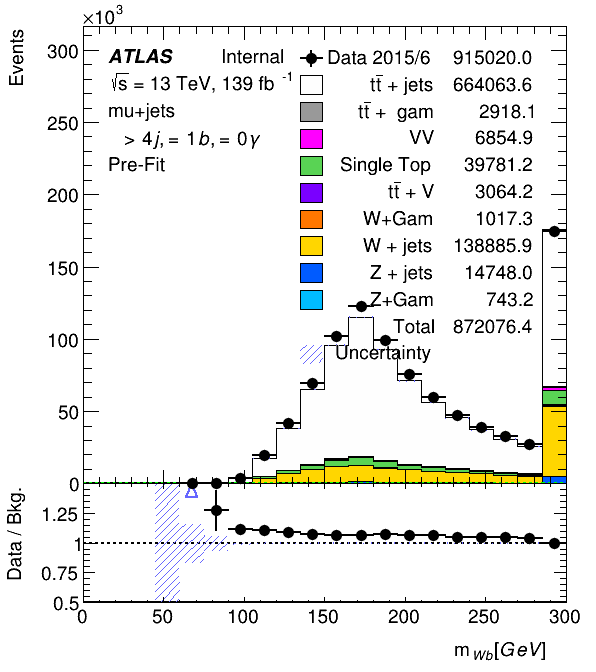
\includegraphics[width=.8\textwidth]{../../Thesis/ThesisImages/RegionPlots/AfterScaling/ControlRegions/HardCodedNormFactor/FCNC_All_mujets/Plots/CR2_SMtop.png}
\end{column}
\begin{column}{0.33\textwidth}
\begin{itemize}
\item Validation Region
\end{itemize}
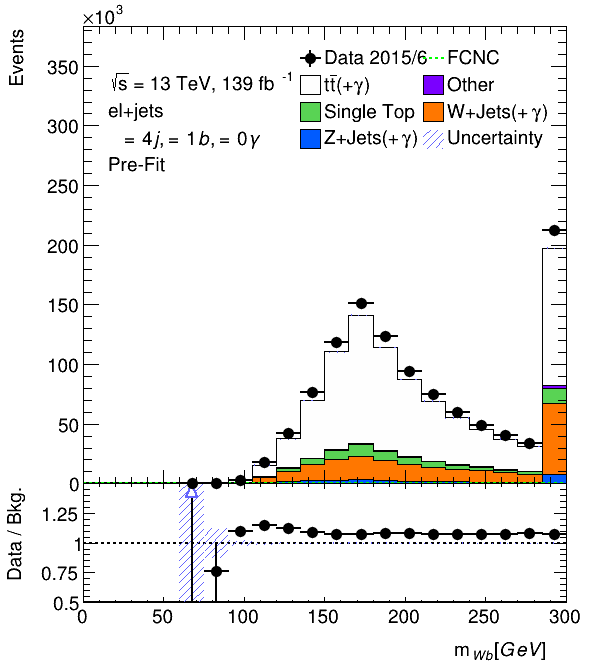
\includegraphics[width=.8\textwidth]{../../Thesis/ThesisImages/RegionPlots/AfterScaling/ControlRegions/HardCodedNormFactor/FCNC_All_ejets/Plots/VR3_SMtop.png} \\
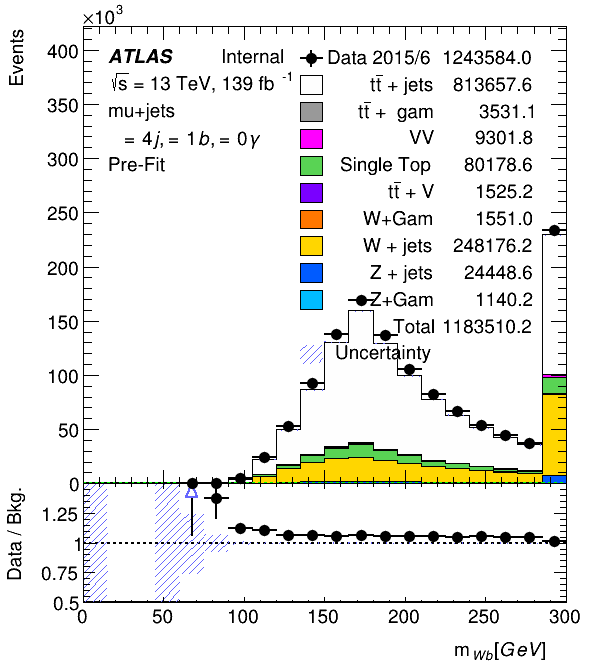
\includegraphics[width=.8\textwidth]{../../Thesis/ThesisImages/RegionPlots/AfterScaling/ControlRegions/HardCodedNormFactor/FCNC_All_mujets/Plots/VR3_SMtop.png}
\end{column}
\end{columns}
}


\frame{\frametitle{0 Photon Regions: VR before/after SF, electron channel}
\begin{columns}
\begin{column}{0.02\textwidth}
\rotatebox{90}{After SF \qquad  Before SF} 
%\rotatebox{90}{Muon Channel        } 
\end{column}
\begin{column}{0.33\textwidth}
\begin{itemize}
\item  $n_\text{bjets}$
\end{itemize}
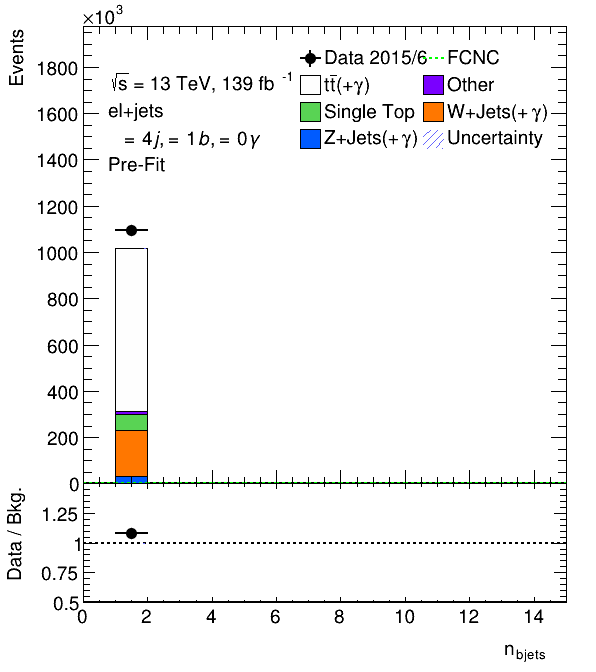
\includegraphics[width=.8\textwidth]{../../Thesis/ThesisImages/RegionPlots/AfterScaling/ControlRegions/HardCodedNormFactor/FCNC_All_ejets/Plots/VR3_nbjet.png} \\
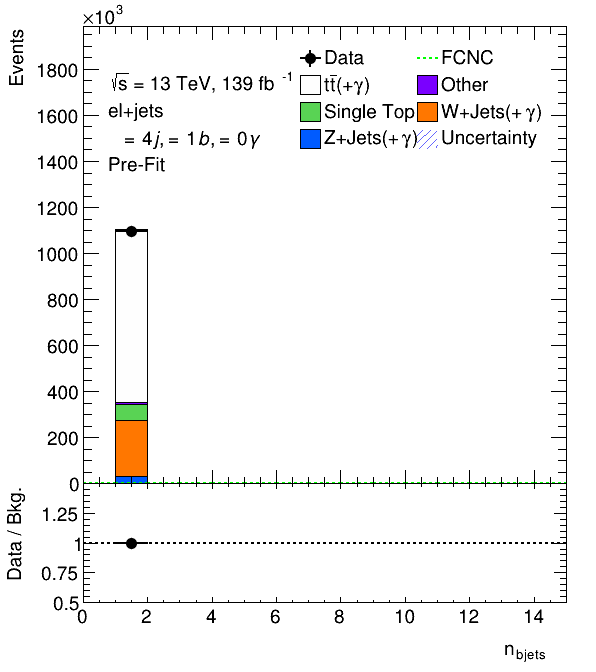
\includegraphics[width=.8\textwidth]{../../Thesis/ThesisImages/RegionPlots/AfterScaling/ControlRegions/HardCodedNormFactor/WithSF/FCNC_All_ejets/Plots/VR3_nbjet.png} 
\end{column}
\begin{column}{0.33\textwidth}
\begin{itemize}
\item Lead Jet $p_T$
\end{itemize}
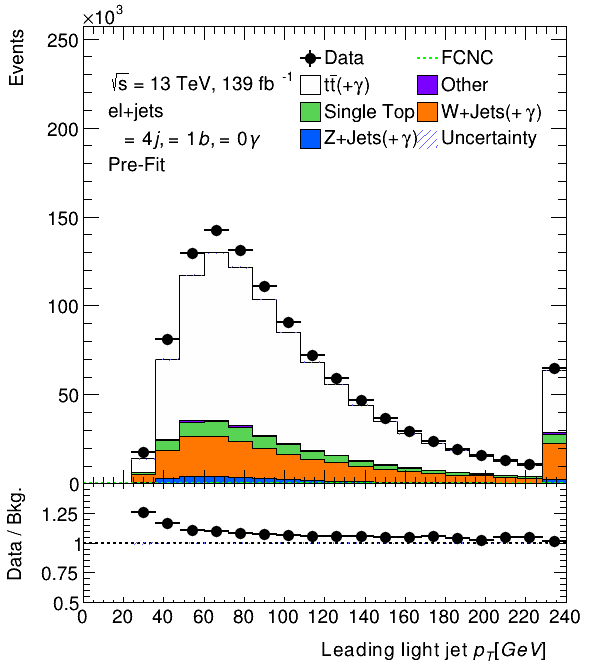
\includegraphics[width=.8\textwidth]{../../Thesis/ThesisImages/RegionPlots/AfterScaling/ControlRegions/HardCodedNormFactor/FCNC_All_ejets/Plots/VR3_jet0_pt.png} \\
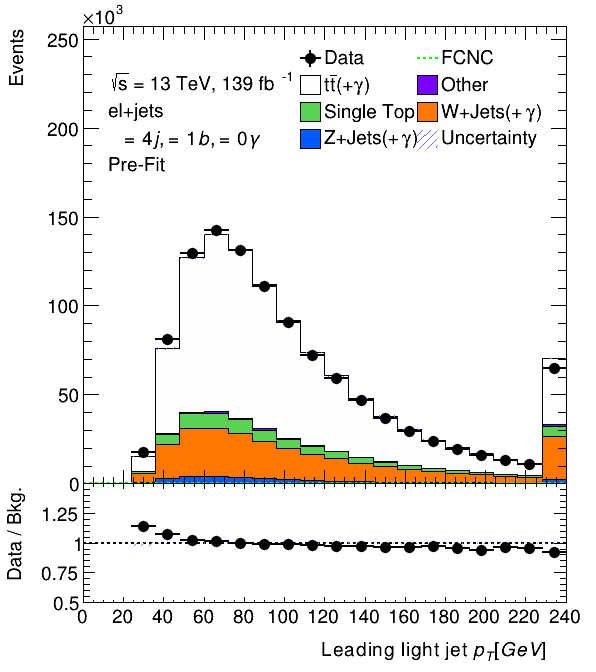
\includegraphics[width=.8\textwidth]{../../Thesis/ThesisImages/RegionPlots/AfterScaling/ControlRegions/HardCodedNormFactor/WithSF/FCNC_All_ejets/Plots/VR3_jet0_pt.png} 
\end{column}
\begin{column}{0.33\textwidth}
\begin{itemize}
\item $m_{Wb}$
\end{itemize}
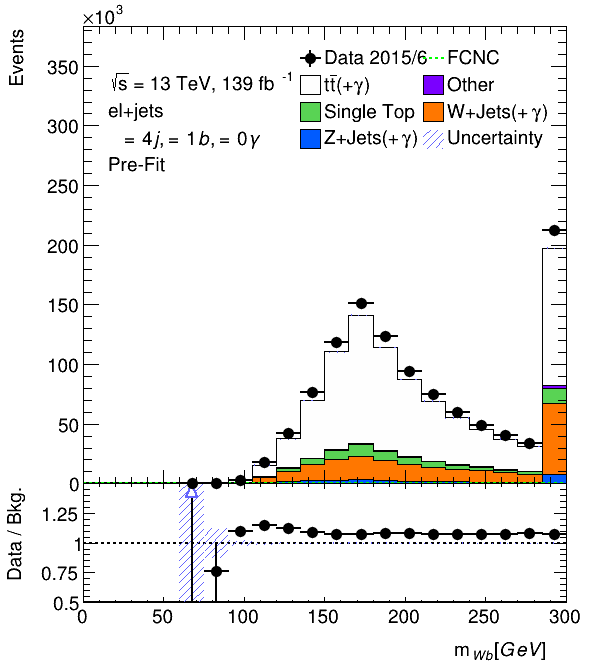
\includegraphics[width=.8\textwidth]{../../Thesis/ThesisImages/RegionPlots/AfterScaling/ControlRegions/HardCodedNormFactor/FCNC_All_ejets/Plots/VR3_SMtop.png} \\
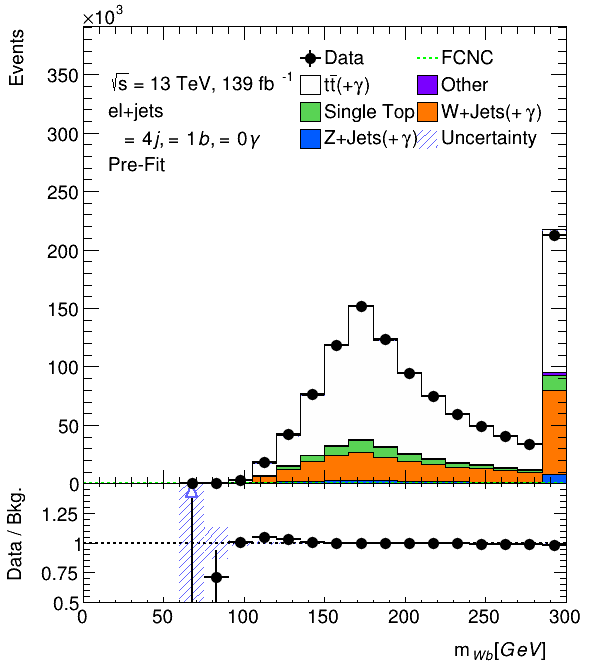
\includegraphics[width=.8\textwidth]{../../Thesis/ThesisImages/RegionPlots/AfterScaling/ControlRegions/HardCodedNormFactor/WithSF/FCNC_All_ejets/Plots/VR3_SMtop.png} 
\end{column}
\end{columns}
}


\subsection{Fake Rates}
\frame{\frametitle{$e\rightarrow \gamma$ Fake Rate Object Selection}
\begin{itemize}
\item Want to calculate fake rate in events which could enter the signal region.
\item Create 2 control regions: $Z\rightarrow ee$ and $Z\rightarrow e \gamma$
\item Require:
	\begin{itemize}
	\item Common Object Selection (MET,Jets,Triggers, etc.)
%	\item Exactly 1Bjet
	\item $Z\rightarrow ee:$ 2 Opposite Sign Electrons, 86.1 GeV $< m_{e^+ e^-} <$96.1 GeV
	\item $Z\rightarrow e\gamma :$1 Electron, $\geq$1 Photon,  86.1 GeV $< m_{e \gamma} <$96.1 GeV

	\end{itemize}
\item Tag and Probe Method used 

\end{itemize}
}

\frame{\frametitle{$e\rightarrow \gamma$ Scale Factor}
\[ \text{FR}^{\text{e-fake}}=\frac{N_{e,\gamma}}{N_{e,e}}\]

\[  \text{SF}^{\text{e-fake}}_{\text{FR}} = \frac{\text{FR}^{\text{e-fake}}_{\text{data}}}{\text{FR}^{\text{e-fake}}_{\text{MC}}}\]
This scale factor is calculated for converted and unconverted photons as well as in bins of $\eta$ and $\phi$
\begin{itemize}
\item Converted photons pair produce before the ECAL leaving tracks in the Inner Detector
\item Unconverted photons only pair produce inside of the ECAL
\end{itemize}
}

\frame{\frametitle{$e\rightarrow \gamma$ 2D Fake Rates}
\begin{columns}
\begin{column}{0.55\textwidth}
\begin{itemize}
\item Converted $\gamma$
\end{itemize}
\includegraphics[width=.95\textwidth]{../../Thesis/ThesisImages/2DConverted.png}
%\includegraphics[width=.95\textwidth]{../../Thesis/ThesisImages/SearchStrategy/FakeRates/2DConverted.png}
\end{column}
\begin{column}{0.55\textwidth}
\begin{itemize}
\item Unconverted $\gamma$
\end{itemize}
\includegraphics[width=.95\textwidth]{../../Thesis/ThesisImages/2DUnconverted.png}
%\includegraphics[width=.95\textwidth]{../../Thesis/ThesisImages/SearchStrategy/FakeRates/2DUnconverted.png}
\end{column}
\end{columns} 
}


\frame{\frametitle{$j\rightarrow \gamma$ Fake Rates}
Majority of hadronic fake photons are from $t\bar{t}$ events where a final state jet radiates a non-prompt photon.  Similarly  radiated photons for W+jets and single top processes can enter the signal region through the radiation of a non-prompt photon. \\
\begin{centering}
\includegraphics[width=.5\textwidth]{../../Thesis/ThesisImages/SearchStrategy/ABCDpictoral.png}\\
\end{centering}
}

\frame{\frametitle{$j\rightarrow \gamma$ ABCD Method}
\begin{columns}
\begin{column}{0.48\textwidth}
\[\frac{N_D^{\text{h-fake}}}{N_C^{\text{h-fake}}}=\frac{N_A^{\text{h-fake}}}{N_B^{\text{h-fake}}}
\text{ and }
\frac{N_D^{\text{h-fake}}}{N_A^{\text{h-fake}}}=\frac{N_C^{\text{h-fake}}}{N_B^{\text{h-fake}}}
\]
Want uncorrelated variables, use a correction factor to account to ensure closure\linespread{1.5}
\[\theta_{\text{MC}}=\frac
{\sfrac{N_\text{D,MC}^{\text{h-fake}}}{N_\text{C,MC}^{\text{h-fake}}}}
{\sfrac{N_\text{A,MC}^{\text{h-fake}}}{N_\text{B,MC}^{\text{h-fake}}}}\]
\[N_\text{D,est.}^{\text{h-fake}} = \frac{N_\text{A,data}^{\text{h-fake}}\times N_\text{C,data}^{\text{h-fake}}}{N_\text{B,data}^{\text{h-fake}}}\times \theta_\text{MC}
\]
\end{column}
\begin{column}{0.48\textwidth}
\includegraphics[width=.95\textwidth]{../../Thesis/ThesisImages/SearchStrategy/ABCDpictoral.png}
\[\text{SF}^\text{h-fake} = \frac{N^\text{h-fake}_\text{D,est.}}{N^\text{h-fake}_\text{D,MC}}
\]
\end{column}
\end{columns}
}


%
\frame{\frametitle{}
\begin{columns}
\begin{column}{0.02\textwidth}
\rotatebox{90}{$\mu$ channel  \qquad \qquad $e$ channel \qquad} 
%\rotatebox{90}{Muon Channel        } 
\end{column}
\begin{column}{0.48\textwidth}
\begin{itemize}
\item Converted Photons
%\item  MCee integral small range: 424,051.  - Vgam: 429789 - All 430225
%\item DATAee integral small range: 468,832
%\item MCeg integral small range: 110822     - Vgam: 115066 - All 152420
%\item DATAeg integral small range: 118198
\end{itemize}
\includegraphics[width=.8\textwidth]{../../Thesis/ThesisImages/SearchStrategy/ABCD/ejetsConverted.png} \\
\includegraphics[width=.8\textwidth]{../../Thesis/ThesisImages/SearchStrategy/ABCD/mujetsConverted.png}
\end{column}
\begin{column}{0.48\textwidth}
\begin{itemize}
\item Unconverted Photons
\end{itemize}
\includegraphics[width=.8\textwidth]{../../Thesis/ThesisImages/SearchStrategy/ABCD/ejetsUnconverted.png} \\
\includegraphics[width=.8\textwidth]{../../Thesis/ThesisImages/SearchStrategy/ABCD/mujetsUnconverted.png}
\end{column}
\end{columns}
\begin{table}[h]
\begin{center}
{\renewcommand{\arraystretch}{1.2}
\begin{tabular}{c|c|c}
\hline
Channel:     & Converted& Unconverted  \\  \hline 
Electron Channel  & $1.28\pm 0.34$     &   $1.99 \pm 0.52$	\\ 
Muon Channel        & $1.23 \pm 0.50$   &   $2.27 \pm 0.92$\\ \hline %Change Put in post fit values
\end{tabular}
}
\end{center}
\end{table}
}



\frame{\frametitle{Post SF Preselection Objects}

\begin{columns}
\begin{column}{0.02\textwidth}

\rotatebox{90}{Muon Channel \qquad  Electron Channel} 
%\rotatebox{90}{Muon Channel        } 
\end{column}
\begin{column}{0.33\textwidth}
\begin{itemize}
\item  Leading Jet $p_T$
\end{itemize}
\includegraphics[width=.8\textwidth]{../../Thesis/ThesisImages/RegionPlots/FinalRegions/presel/FCNC_All_ejets/Plots/PreSel_jet0_pt.png} \\
\includegraphics[width=.8\textwidth]{../../Thesis/ThesisImages/RegionPlots/FinalRegions/presel/FCNC_All_mujets/Plots/PreSel_jet0_pt.png}
\end{column}
\begin{column}{0.33\textwidth}
\begin{itemize}
\item Photon $p_T$
\end{itemize}
\includegraphics[width=.8\textwidth]{../../Thesis/ThesisImages/RegionPlots/FinalRegions/presel/FCNC_All_ejets/Plots/PreSel_ph_pt.png} \\
\includegraphics[width=.8\textwidth]{../../Thesis/ThesisImages/RegionPlots/FinalRegions/presel/FCNC_All_mujets/Plots/PreSel_ph_pt.png}
\end{column}
\begin{column}{0.33\textwidth}
\begin{itemize}
\item Lepton $p_T$
\end{itemize}
\includegraphics[width=.8\textwidth]{../../Thesis/ThesisImages/RegionPlots/FinalRegions/presel/FCNC_All_ejets/Plots/PreSel_lep_pt.png}\\
\includegraphics[width=.8\textwidth]{../../Thesis/ThesisImages/RegionPlots/FinalRegions/presel/FCNC_All_mujets/Plots/PreSel_lep_pt.png}
\end{column}
\end{columns}

}

\subsection{Neural Network Optimization}
\frame{\frametitle{Neural Networks}
\begin{itemize}
\item Advanced pattern recognition used to classify events
\item A dense neural network is used with various low and high level variable inputs
\item Supervised learning used to approximate any multidimensional function
\end{itemize}
\centering
\includegraphics[width=0.7\textwidth]{Images/neural_net2.jpeg}
\captionof{figure}{\href{http://cs231n.github.io/neural-networks-1/}{[Ref: Neural Network]}}
}

\frame{\frametitle{Neural Network Model Inputs}
\begin{itemize}
\item Using keras on top of tensorflow various network architectures were tested
\item Networks are set up with 1 input layer, 2 hidden layers of 10 nodes, and 1 output node
\item Each hidden layer has 20\% dropout to prevent overtraining by removing codependency between nodes
\item Batch size of 100 used and each network is allowed 200 epochs (with patience=50), all models converge and end early with reasonable batch sizes
\item Optimizer: Adam
\item Loss Function: Binary Cross Entropy
\end{itemize}
}

\frame{\frametitle{Neural Network Example Outputs}
e+jets Channel Example
\begin{columns}
\begin{column}{0.5\textwidth}
\includegraphics[width=.85\textwidth]{../../Thesis/ThesisImages/SearchStrategy/{HiddenLayerStudiesBR0.002}/BestResults/btag77/ejetsboth2hidnpart0accuarcy.png} \\
\includegraphics[width=.85\textwidth]{../../Thesis/ThesisImages/SearchStrategy/{HiddenLayerStudiesBR0.002}/BestResults/btag77/ejetsboth2hidnpart0loss.png}
\end{column}
\begin{column}{0.5\textwidth}

\includegraphics[width=.85\textwidth]{../../Thesis/ThesisImages/SearchStrategy/{HiddenLayerStudiesBR0.002}/BestResults/btag77/ejetsboth2hidnpart0sigbkg.png} \\
\includegraphics[width=.85\textwidth]{../../Thesis/ThesisImages/SearchStrategy/{HiddenLayerStudiesBR0.002}/BestResults/btag77/significanceejetsboth2hidnpart02.png}
\end{column}

\end{columns}
}

%%%%%%%%%%%FIX FIX fix Fix Fix fix
\frame{\frametitle{}
Explain about VRs, closer to SR than preselec
Maybe show NN output in VR2\\
\includegraphics[width=.4\textwidth]{../../Thesis/ThesisImages/RegionPlots/FinalRegions/presel/FCNC_All_ejets/Plots/PreSel_NNejet.png}
\includegraphics[width=.4\textwidth]{../../Thesis/ThesisImages/RegionPlots/FinalRegions/presel/FCNC_All_mujets/Plots/PreSel_NNmujet.png}
}

\subsection{Validation Region and Signal Region Fits}


\frame{\frametitle{Validation Regions: $W+\text{jets}+\gamma$}
\begin{columns}
\begin{column}{0.02\textwidth}
\rotatebox{90}{Muon Channel \qquad  Electron Channel} 
%\rotatebox{90}{Muon Channel        } 
\end{column}
\begin{column}{0.33\textwidth}
\begin{itemize}
\item  $\gamma p_T$
\end{itemize}
\includegraphics[width=.8\textwidth]{../../Thesis/ThesisImages/RegionPlots/BeforeScaling/PhotonRegions/FCNC_All_ejets/Plots/VR1_ph_pt.png} \\
\includegraphics[width=.8\textwidth]{../../Thesis/ThesisImages/RegionPlots/BeforeScaling/PhotonRegions/FCNC_All_mujets/Plots/VR1_ph_pt.png} 
\end{column}
\begin{column}{0.33\textwidth}
\begin{itemize}
\item Lead Jet $p_T$
\end{itemize}
\includegraphics[width=.8\textwidth]{../../Thesis/ThesisImages/RegionPlots/BeforeScaling/PhotonRegions/FCNC_All_ejets/Plots/VR1_jet0_pt.png} \\
\includegraphics[width=.8\textwidth]{../../Thesis/ThesisImages/RegionPlots/BeforeScaling/PhotonRegions/FCNC_All_mujets/Plots/VR1_jet0_pt.png} 
\end{column}
\begin{column}{0.33\textwidth}
\begin{itemize}
\item $m_{Wb}$
\end{itemize}
\includegraphics[width=.8\textwidth]{../../Thesis/ThesisImages/RegionPlots/BeforeScaling/PhotonRegions/FCNC_All_ejets/Plots/VR1_jet0_pt.png} \\
\includegraphics[width=.8\textwidth]{../../Thesis/ThesisImages/RegionPlots/BeforeScaling/PhotonRegions/FCNC_All_mujets/Plots/VR1_jet0_pt.png} 
\end{column}
\end{columns}
}

\frame{\frametitle{Validation Regions: $t\bar{t}+\text{jets}+\gamma$}
\begin{columns}
\begin{column}{0.02\textwidth}
\rotatebox{90}{Muon Channel \qquad  Electron Channel} 
%\rotatebox{90}{Muon Channel        } 
\end{column}
\begin{column}{0.33\textwidth}
\begin{itemize}
\item  $\gamma p_T$
\end{itemize}
\includegraphics[width=.8\textwidth]{../../Thesis/ThesisImages/RegionPlots/BeforeScaling/PhotonRegions/FCNC_All_ejets/Plots/VR2_ph_pt.png} \\
\includegraphics[width=.8\textwidth]{../../Thesis/ThesisImages/RegionPlots/BeforeScaling/PhotonRegions/FCNC_All_mujets/Plots/VR2_ph_pt.png} 
\end{column}
\begin{column}{0.33\textwidth}
\begin{itemize}
\item Lead Jet $p_T$
\end{itemize}
\includegraphics[width=.8\textwidth]{../../Thesis/ThesisImages/RegionPlots/BeforeScaling/PhotonRegions/FCNC_All_ejets/Plots/VR2_jet0_pt.png} \\
\includegraphics[width=.8\textwidth]{../../Thesis/ThesisImages/RegionPlots/BeforeScaling/PhotonRegions/FCNC_All_mujets/Plots/VR2_jet0_pt.png} 
\end{column}
\begin{column}{0.33\textwidth}
\begin{itemize}
\item $m_{Wb}$
\end{itemize}
\includegraphics[width=.8\textwidth]{../../Thesis/ThesisImages/RegionPlots/BeforeScaling/PhotonRegions/FCNC_All_ejets/Plots/VR2_jet0_pt.png} \\
\includegraphics[width=.8\textwidth]{../../Thesis/ThesisImages/RegionPlots/BeforeScaling/PhotonRegions/FCNC_All_mujets/Plots/VR2_jet0_pt.png} 
\end{column}
\end{columns}
}


\frame{\frametitle{Analysis}
}
\frame{\frametitle{Pre-fit Signal Region Plots}
\begin{columns}
\begin{column}{0.02\textwidth}
\rotatebox{90}{Muon channel  \qquad \qquad Electron channel \qquad} 
%\rotatebox{90}{Muon Channel        } 
\end{column}
\begin{column}{0.48\textwidth}
$m_{q\gamma}$\\
\includegraphics[width=.6\textwidth]{../../Thesis/ThesisImages/RegionPlots/FinalRegions/Systematics/FCNC_All_ejets/Plots/SR_mqph.png} \\
\includegraphics[width=.6\textwidth]{../../Thesis/ThesisImages/RegionPlots/FinalRegions/Systematics/PhotonPT/FCNC_All_mujets/Plots/SRmu_mqph.png}
\end{column}
\begin{column}{0.48\textwidth}
$\gamma p_T$ \\
\includegraphics[width=.6\textwidth]{../../Thesis/ThesisImages/RegionPlots/FinalRegions/Systematics/FCNC_All_ejets/Plots/SR_ph_pt.png} \\
\includegraphics[width=.6\textwidth]{../../Thesis/ThesisImages/RegionPlots/FinalRegions/Systematics/PhotonPT/FCNC_All_mujets/Plots/SRmu_ph_pt.png}
\end{column}
\end{columns}
}
\frame{\frametitle{Systematic Uncertainties - Nuisance Parameters}
}
\frame{\frametitle{Post-fit Signal Region Plots}
\begin{columns}
\begin{column}{0.02\textwidth}
\rotatebox{90}{Muon channel  \qquad \qquad Electron channel \qquad} 
%\rotatebox{90}{Muon Channel        } 
\end{column}
\begin{column}{0.48\textwidth}
$m_{q\gamma}$\\
\includegraphics[width=.6\textwidth]{../../Thesis/ThesisImages/RegionPlots/FinalRegions/Systematics/FCNC_All_ejets/Plots/SR_mqph_postFit.png} \\
\includegraphics[width=.6\textwidth]{../../Thesis/ThesisImages/RegionPlots/FinalRegions/Systematics/PhotonPT/FCNC_All_mujets/Plots/SRmu_mqph_postFit.png}
\end{column}
\begin{column}{0.48\textwidth}
$\gamma p_T$ \\
\includegraphics[width=.6\textwidth]{../../Thesis/ThesisImages/RegionPlots/FinalRegions/Systematics/FCNC_All_ejets/Plots/SR_ph_pt_postFit.png} \\
\includegraphics[width=.6\textwidth]{../../Thesis/ThesisImages/RegionPlots/FinalRegions/Systematics/PhotonPT/FCNC_All_mujets/Plots/SRmu_ph_pt_postFit.png}
\end{column}
\end{columns}
}

\frame{\frametitle{$\text{CL}_{s}$ Method - Limit Setting}
}
\frame{\frametitle{Result - Limit on BR($t\rightarrow q\gamma$)}
\begin{figure}[ht!]
	\centering
	\includegraphics[width=0.5\columnwidth]{../../Thesis/ThesisImages/RegionPlots/FinalRegions/Systematics/MQGamEJetPHptMJet/LimitPlot.png}
\end{figure}
\begin{table}[h!]
\begin{center}
{\renewcommand{\arraystretch}{1.2}
\begin{tabular}{ccc}
Channel  	&  Obs. Limit		& Exp. Limit	  \\  \hline 
e+jets	& $1.19\times10^{-4}$ 	& $1.31(^{+0.47}_{-0.36})\times10^{-4}$ 	\\ 
$\mu$+jets	& $1.53\times10^{-4}$ 	& $1.42(^{+0.51}_{-0.39})\times10^{-4}$ 	\\ 
Combined	& $0.96\times10^{-4}$ 	& $1.10(^{+0.43}_{-0.30})\times10^{-4}$ 	\\
\end{tabular}
}
\end{center}
\end{table}
}

\section{Conclusion}
%%%%%%%%%%%%%%%%%%%%%%%%%%%%%%%%%%%%%%%%%%%%%%%%%%%%%%%%%%%%%%%%%
%%%%%%%%%%%%%%%%%%%%%%%%%%%%%%%%%%%%%%%%%%%%%%%%%%%%%%%%%%%%%%%%%%

\frame{\frametitle{Conclusions}
\begin{itemize}
\item Limits have been set on the process $t\rightarrow q \gamma$
\item Neural network implementation improved result by up to 30\% compared to stats only improvement
\end{itemize}
}

\frame{\frametitle{Thank You}
\begin{centering}
Special thank you to my committee: \\
David Strom (Chair) \\
Spencer Chang \\
Dev Sinha \\
My Advisor: Jim Brau \\
\end{centering}
}
\frame{\frametitle{Questions?}
\centering
\includegraphics[width=.7\textwidth]{../../Thesis/ThesisImages/JasonAtATLAS.jpg}
}



%%%%%%%%%%%%%%%%%%%%%%%%%%%%%%%%%%%%%%%%%%%%%%%%%%%%%%%%%%%%%%%%
%%%%%%%%%%%%%%%%%%%%%%%%%%%%%%%%%%%%%%%%%%%%%%%%%%%%%%%%%%%%%%%%
%%%%%%%%%%%%%%%%%%%%%%%%%%%%%%%%%%%%%%%%%%%%%%%%%%%%%%%%%%%%%%%%
%%%%%%%%%%%%%%%%%%%%%%%%%%%%%%%%%%%%%%%%%%%%%%%%%%%%%%%%%%%%%%%%
%%%%%%%%%%%%%%%%%%%%%%%%%%%%%%%%%%%%%%%%%%%%%%%%%%%%%%%%%%%%%%%%
%%%%%%%%%%%%%%%%%%%%%%%%%%%%%%%%%%%%%%%%%%%%%%%%%%%%%%%%%%%%%%%%
%%%%%%%%%%%%%%%%%%%%%%%%%%%%%%%%%%%%%%%%%%%%%%%%%%%%%%%%%%%%%%%%
%%%%%%%%%%%%%%%%%%%%%%%%%%%%%%%%%%%%%%%%%%%%%%%%%%%%%%%%%%%%%%%%

\appendix
\section{Backup}
\frame{\frametitle{Backup}
}
\frame{\frametitle{FCNC Diagrams}
\centering
\includegraphics[width=.4\textwidth]{../../Thesis/ThesisImages/Theory/FCNCLoop.png}
\includegraphics[width=.4\textwidth]{../../Thesis/ThesisImages/penguinFCNC.png}
}



\frame{\frametitle{Neural Network Model Inputs}
\centering
\scalebox{0.8}{ $\text{Separation} = \sum_{i}^{bins} \frac {n_{s i}-n_{b i}}{n_{s i}+n_{b i}}$}
\begin{columns}
\begin{column}{0.48\textwidth}
\centering
mu+jets channel\\
\scalebox{0.6}{\begin{tabular}{cc}
Variable & Separation \\
\hline
photon0iso & 41.18 \\
mqgam & 28.27 \\
photon0pt & 24.07 \\
mtSM & 11.60 \\
mlgam & 7.56 \\
deltaRjgam & 5.64 \\
deltaRbl & 4.42 \\
MWT & 3.34 \\
ST & 3.30 \\
nuchi2 & 3.12 \\
jet0pt & 2.81 \\
njets & 2.07 \\
smchi2 & 1.89 \\
wchi2 & 1.87 \\
jet0e & 1.52 \\
deltaRlgam & 1.17 \\
leptone & 0.87 \\
deltaRjb & 0.86 \\
met & 0.68 \\
bjet0pt & 0.52 \\
leptoniso & 0.27 \\
\end{tabular}
}
\end{column}
\begin{column}{0.48\textwidth}
\centering
e+jets channel \\
\scalebox{0.6}{\begin{tabular}{c c}
Variable & Separation\\
\hline
photon0pt & 23.14 \\
mqgam & 22.73 \\
photon0iso & 18.70 \\
mtSM & 11.02 \\
mlgam & 9.53 \\
deltaRbl & 5.00 \\
deltaRjgam & 4.60 \\
ST & 3.83 \\
MWT & 3.16 \\
jet0pt & 2.47 \\
njets & 1.70 \\
nuchi2 & 1.59 \\
deltaRlgam & 1.40 \\
wchi2 & 1.33 \\
smchi2 & 1.09 \\
deltaRjb & 0.88 \\
leptone & 0.85 \\
leptoniso & 0.56 \\
bjet0pt & 0.50 \\
met & 0.47 \\
\end{tabular}
}
\end{column}
\end{columns}
}

\frame{\frametitle{Input Variables}
['photon0iso','photon0pt','mqgam','mlgam','mtSM','deltaRjgam','deltaRbl',\\
'MWT','ST','njets','wchi2','jet0pt','deltaRlgam','leptone','met','bjet0pt']


}


\frame{\frametitle{A Couple BSM Diagrams}
\centering
\includegraphics[width=1.\textwidth]{../../Thesis/ThesisImages/BSMDiagrams.png}
}

\frame{\frametitle{Jets/AntiKT}

\[ d_{ij} = min(\frac{1}{p_{ti}^2},\frac{1}{p_{tj}^2}) \frac{\Delta_{ij}^2}{R^2}
\]
\[ d_{iB} = \frac{1}{p_{ti}^2}
\]
\[ \Delta_{ij}^2 = (\eta_i -\eta_j )^2 + (\phi_i - \phi_j )^2
\]
\begin{itemize}
\item Find minimum of entire set of $\{ d_{ij},d_{iB} \}$
\item If $d_{ij}$ is the minimum particles i,j are combined into one particle and removed from the list of particles
\item If $d_{iB}$ is the minimum i is labelled as a final jet and removed from the list of particles
\item Repeat until all particles are part of a jet with distance between jet axes $\Delta_{ij}$ is greater than R
\end{itemize}
}
\frame{\frametitle{B-tagging}
\begin{columns}
\begin{column}{0.5\textwidth}
\begin{itemize}
\item B Hadrons travel a measureable distance before decay
\item Tracks originate from outside of interaction point (Seconday Vertex)
\item Backtracking tracks in displaced vertex gives an impact parameter
\item Decay chain MVA attempts to reconstruct decay of the jet
\item Outputs of these algorithms used in a BDT to determine if a Jet is from a b-quark
\end{itemize}
\end{column}
\begin{column}{0.5\textwidth}
\centering
\includegraphics[height=.65\textheight]{../../Thesis/ThesisImages/Simulation/B-tagging_diagram.png}
\end{column}
\end{columns}
}


\frame{\frametitle{Jet Algorithms}
\centering
\includegraphics[width=.7\textwidth]{../../Thesis/ThesisImages/Simulation/VarJetAlgs.png}
\begin{itemize}
\item IR Safety: Adding soft emission particle does not change final jet configuration
\item Collinear Safety: Splitting a jet into 2 collinear jets yields the same result, jet size does not matter
\end{itemize}
}
\frame{\frametitle{Jet Algorithms}
\centering
\includegraphics[width=.7\textwidth]{../../Thesis/ThesisImages/IRCollinearSafety.png} \\
Courtesy - John Myers
}

\frame{\frametitle{What's in the data?}
\begin{columns}
\begin{column}{0.5\textwidth}
\centering 
\includegraphics[width=1.\textwidth]{../../Thesis/ThesisImages/HardScatCrosSecs.png}
\end{column}
\begin{column}{0.5\textwidth}
\begin{itemize}
\item The number of events we see is $N=\sigma L$
\item $\sigma_{t\bar{t}}=$ 831.76pb
\item $N_{t\bar{t}} \approx 116x10^6$
\item $N_{tot} \approx 14x10^{15}$ events produced during the 13TeV data runs
\end{itemize}
\end{column}
\end{columns}
}

\frame{egamma fake rate Data and MC \frametitle{$m_{ee}, m_{e\gamma}$}
\begin{columns}
\begin{column}{0.02\textwidth}
\rotatebox{90}{$m_{e\gamma}$ \qquad \qquad \qquad $m_{ee}$\qquad} 
%\rotatebox{90}{Muon Channel        } 
\end{column}
\begin{column}{0.48\textwidth}
\begin{itemize}
\item Data
\end{itemize}
\includegraphics[width=.85\textwidth]{Images/Dataee.png} \\
\includegraphics[width=.85\textwidth]{Images/Dataeg.png}
\end{column}
\begin{column}{0.48\textwidth}
\begin{itemize}
\item Monte Carlo
\end{itemize}
\includegraphics[width=.85\textwidth]{Images/MCVgamee.png} \\
\includegraphics[width=.85\textwidth]{Images/MCVgameg.png}
\end{column}
\end{columns}
}
\frame{\frametitle{$e\rightarrow \gamma$ Data and MC Distributions}
\begin{columns}
\begin{column}{0.02\textwidth}
\rotatebox{90}{MC \qquad \qquad Data\qquad} 
%\rotatebox{90}{Muon Channel        } 
\end{column}
\begin{column}{0.32\textwidth}
\begin{itemize}
\item Probe $e$
\end{itemize}
\includegraphics[width=.95\textwidth]{../../Thesis/ThesisImages/SearchStrategy/FakeRates/2dEEptDa.png} \\
\includegraphics[width=.95\textwidth]{../../Thesis/ThesisImages/SearchStrategy/FakeRates/2dEEptMC.png} \\
\end{column}
\begin{column}{0.32\textwidth}
\begin{itemize}
\item Converted $\gamma$
\end{itemize}
\includegraphics[width=.95\textwidth]{../../Thesis/ThesisImages/SearchStrategy/FakeRates/2dEPConvertedptDa.png} \\
\includegraphics[width=.95\textwidth]{../../Thesis/ThesisImages/SearchStrategy/FakeRates/2dEPConvertedptMC.png}
\end{column}
\begin{column}{0.32\textwidth}
\begin{itemize}
\item Unconverted $\gamma$
\end{itemize}
\includegraphics[width=.95\textwidth]{../../Thesis/ThesisImages/SearchStrategy/FakeRates/2dEPUnconvertedptDa.png} \\
\includegraphics[width=.95\textwidth]{../../Thesis/ThesisImages/SearchStrategy/FakeRates/2dEPUnconvertedptMC.png}
\end{column}
\end{columns}
}

\frame{\frametitle{Neural Network Optimizers}
\begin{itemize}
\item Various optimization functions can be used, I make use of Adam (Adaptive Moment Estimation)
\begin{itemize}
\item Adam computes adaptive learning rates for every parameter and stores a history of the parameters used to calculate the next step
\item Stores first (mean) and second (uncentered variance) moments of the gradients used during training
\item Converges very fast and is less computationally intensive
\end{itemize}
\end{itemize}
\centering
\includegraphics[width=0.35\textwidth]{Images/AdamComparison.png}
\captionof{figure}{\href{https://machinelearningmastery.com/adam-optimization-algorithm-for-deep-learning/}{[Ref:Machine Learning Mastry]}}
}
\frame{\frametitle{Neural Network Example Outputs}
mu+jets Channel Example
\begin{columns}
\begin{column}{0.5\textwidth}
\includegraphics[width=.85\textwidth]{../../Thesis/ThesisImages/SearchStrategy/{HiddenLayerStudiesBR0.002}/BestResults/btag77/mujetsboth2hidnpart0accuarcy.png} \\
\includegraphics[width=.85\textwidth]{../../Thesis/ThesisImages/SearchStrategy/{HiddenLayerStudiesBR0.002}/BestResults/btag77/mujetsboth2hidnpart0loss.png}
\end{column}
\begin{column}{0.5\textwidth}

\includegraphics[width=.85\textwidth]{../../Thesis/ThesisImages/SearchStrategy/{HiddenLayerStudiesBR0.002}/BestResults/btag77/mujetsboth2hidnpart0sigbkg.png} \\
\includegraphics[width=.85\textwidth]{../../Thesis/ThesisImages/SearchStrategy/{HiddenLayerStudiesBR0.002}/BestResults/btag77/significancemujetsboth2hidnpart02.png}
\end{column}

\end{columns}
}
\frame{\frametitle{Duplicate Event Removal}
}

%\frame{\frametitle{B-tagging}
%\centering
%\includegraphics[height=.8\textheight]{../../Thesis/ThesisImages/SimulationNN/B-tagging_diagram.png}
%}

\frame{\frametitle{}
\[ \mathcal{L}^{eff}_{tq\gamma} = - e \bar{c} \frac{i \sigma^{\mu\nu}q_{\nu}}{m_t}(\lambda^{L}_{ct}P_L + \lambda^{R}_{ct}P_{R}) t A_{\mu} +H.c.
\]
}

\frame{\frametitle{0 Photon Regions: VR before/after SF, muon channel}
\begin{columns}
\begin{column}{0.02\textwidth}
\rotatebox{90}{After SF \qquad  Before SF} 
%\rotatebox{90}{Muon Channel        } 
\end{column}
\begin{column}{0.33\textwidth}
\begin{itemize}
\item  $n_\text{bjets}$
\end{itemize}
\includegraphics[width=.85\textwidth]{../../Thesis/ThesisImages/RegionPlots/AfterScaling/ControlRegions/HardCodedNormFactor/FCNC_All_mujets/Plots/VR3_nbjet.png} \\
\includegraphics[width=.85\textwidth]{../../Thesis/ThesisImages/RegionPlots/AfterScaling/ControlRegions/HardCodedNormFactor/WithSF/FCNC_All_mujets/Plots/VR3_nbjet.png} 
\end{column}
\begin{column}{0.33\textwidth}
\begin{itemize}
\item Lead Jet $p_T$
\end{itemize}
\includegraphics[width=.85\textwidth]{../../Thesis/ThesisImages/RegionPlots/AfterScaling/ControlRegions/HardCodedNormFactor/FCNC_All_mujets/Plots/VR3_jet0_pt.png} \\
\includegraphics[width=.85\textwidth]{../../Thesis/ThesisImages/RegionPlots/AfterScaling/ControlRegions/HardCodedNormFactor/WithSF/FCNC_All_mujets/Plots/VR3_jet0_pt.png} 
\end{column}
\begin{column}{0.33\textwidth}
\begin{itemize}
\item $m_{Wb}$
\end{itemize}
\includegraphics[width=.85\textwidth]{../../Thesis/ThesisImages/RegionPlots/AfterScaling/ControlRegions/HardCodedNormFactor/FCNC_All_mujets/Plots/VR3_SMtop.png} \\
\includegraphics[width=.85\textwidth]{../../Thesis/ThesisImages/RegionPlots/AfterScaling/ControlRegions/HardCodedNormFactor/WithSF/FCNC_All_mujets/Plots/VR3_SMtop.png} 
\end{column}
\end{columns}
}


\end{document}

%36.070


%%% Neural Net Ref: http://cs231n.github.io/neural-networks-1/

% npart0=['photon0_iso','photon0_pt','m_qgam','m_lgam','m_tSM','deltaRjgam','deltaRbl','MWT','S_T','nbjets','njets','w_chi2','jet0_pt','nu_chi2','sm_chi2','deltaRlgam','lepton_e','met','lepton_iso','bjet0_pt']
%all vars

%npart = ['photon0_iso','photon0_pt','m_qgam','m_lgam','m_tSM','deltaRjgam','deltaRbl','MWT','S_T','njets','nbjets','w_chi2','jet0_pt','deltaRlgam','lepton_e','met','bjet0_pt']
%usual npart1

%npart1=['photon0_iso','photon0_pt','deltaRjgam','deltaRbl','MWT','S_T','njets','w_chi2','jet0_pt','deltaRlgam','lepton_e','met','bjet0_pt']
%minimal